%%%%%%%%%%%%%%%%%%%%%%%%%%%%%%%%%%%%%%%%%%%%%%%%%%%%%%%%%%%%%%%%%%%%%%%%%%%%%%%%
\section{Improving PDF fits with lattice-QCD calculations}
\label{sec:projections}
%%%%%%%%%%%%%%%%%%%%%%%%%%%%%%%%%%%%%%%%%%%%%%%%%%%%%%%%%%%%%%%%%%%%%%%%%%%%%%%%

In this section, we provide an estimate of the potential
impact of future lattice-QCD calculations
in global unpolarized and polarized PDF fits.
%
This study is carried out with two publicly available
tools: the Bayesian reweighting
method~\cite{Ball:2011gg,Ball:2010gb} applied to the
NNPDF3.1~\cite{Ball:2017nwa} and NNPDFpol1.1~\cite{Nocera:2014gqa} sets; 
and the Hessian profiling method~\cite{Camarda:2015zba} applied to
HERAPDF2.0 set~\cite{Abramowicz:2015mha}.
%
Both methods allow us to quantify the impact of new measurements
(or of future measurements, if pseudo-data are used) on PDFs without
repeating the global analysis.
%
The main limitation of these methods is that they are maximally reliable
if the amount of information carried in by the new (pseudo-)data is moderate
in comparison to that already included in the fit.

For simplicity, we limit our study to the impact of a subset of the moments 
that can be computed using lattice QCD, focusing on those that can be 
currently calculated with the highest precision.
%
Therefore, we restrict ourselves to the benchmark moments discussed in 
Sec.~\ref{sec:benchmarking}.
%
We also consider pseudo-data based on $x$-space
lattice-QCD calculations from the quasi-PDF approach
discussed in Sec.~\ref{sec:xdependence}.
%
As we show, particularly in the unpolarized case, the
constraining power of direct $x$-space calculations is
superior to that of PDF moments.

\subsection{Impact of lattice calculations of PDF moments}

We start by quantifying the constraining power of projected lattice-QCD 
calculations of PDF moments on both unpolarized and polarized global fits.
%
We define the settings for our study and present our results following
Bayesian reweighting and Hessian profiling, respectively.

% General projections for moments
\subsubsection{Analysis settings}
\label{sec:projections:settings}

The following projection studies aiming to quantify
the impact of present and future lattice-QCD calculations
of PDF moments will be based on the following specific choice
of moments.
%
For the unpolarized case, we will use
\be
  \la x\ra_{u^+}\, , \quad
\la x\ra_{d^+}\, , \quad
\la x\ra_{s^+}\, , \quad
\la x\ra_{g}\, , \quad {\rm and} \quad
\la x\ra_{u^+-d^+} \, ,
\ee
while for the polarized side, we will include instead
the following five moments:
\be
\la 1\ra_{\Delta u^+}\, , \quad
\la 1\ra_{\Delta d^+}\, , \quad
\la 1\ra_{\Delta s^+}\, , \quad
\la x\ra_{\Delta u^--\Delta d^-}\, , \quad {\rm and} \quad
\la 1\ra_{\Delta u^+ - \Delta d^+} \, .
\ee
Recall that Appendix~\ref{app:notation} contains the
explicit definitions and conventions used for these moments.
%
That is,  for the unpolarized case we include
the second moments (momentum fractions) of $q^+$ (with $q=u,d,s$),
of the gluon, and of the isoscalar combination $u^+-d^+$.
%
In the polarized case instead, we include the first moments (which
contribute to the proton spin sum rule) of $\Delta q^+$ (with $q=u,d,s$)
and of the isoscalar combination $g_A=\Delta u^+-\Delta d^+$, as well as
the second moment of the $\Delta u^- - \Delta d^-$ combination.

In the present exercise we will consider three
different scenarios, which we denote
as Scenario A, B, and C respectively, for the total systematic
uncertainty than we associate to lattice
QCD calculations of PDF moments.
%
In Table~\ref{tab:scenarios} we summarize the
values assumed for this total uncertainty
    of the lattice QCD calculation, denoted by $\delta_L$, for each
    of the various unpolarized and polarized PDF moments that enter
    this analysis.
    %
    We emphasize that here, while trying to be reasonably
    realistic, we do not aim to associate a given scenario
    within a specific time-scale for the calculation.
    %
    Our results  merely provide an illustrative guidance about the potential
    constraining power of existing and future lattice QCD calculations
    of PDF  moments in the context
    of a global analysis.
    
    The motivation for our choice of the scenarios
    in Table~\ref{tab:scenarios}
    is rather different from the unpolarized and polarized cases.
    %
    For the polarized fits,
    scenario A assumes that the uncertainties $\delta_L$
    for the lattice QCD calculations
    are on same the ball-park of the current ones, taking as
    representative values for the latter  those from the
    state-of-the-art lattice QCD calculations
    selected for the benchmarking exercise of Sect.~\ref{sec:benchmarking},
    and summarized in Table~\ref{tab:BMpol}.
    %
    Then scenarios B and C represent two possible optimistic scenarios for the
    future improvement of these systematic uncertainties, where these are decreased
    by roughly a factor 2 and a factor 4 with respect current values.
    
    On the other hand, for the unpolarized case scenario A is based on values
    of $\delta_L^{(i)}$ already rather smaller than the typical
    uncertainties that affect state-of-the-art calculations, see Table~\ref{tab:BMunp}.
    %
    The reason is that we have verified that including the lattice-QCD pseudo-data
    assuming uncertainties of similar size as those of Table~\ref{tab:BMunp}
    leaves the PDFs essentially unchanged, and only once the uncertainties
    $\delta_L^{(i)}$ are significantly reduced that we start to obtain a reduction
    of the uncertainties from the global fit.
    %
    The only connection with the uncertainties of the calculations in Table~\ref{tab:BMunp}
    is that we assume that $\delta_L^{(i)}$ is typically larger for $\la x\ra_{s^+}$
        and $\la x\ra_{u^+-d^+}$ as compared to the other moments.

    We also note that
    a total systematic error of $\delta_L^{(i)}\sim 1\%$
    is probably the best that one can achieve
    within a lattice-QCD calculation even in principle, since at that level several other
    effects, such as QED corrections,
    become relevant and these are much more difficult
    to deal with.
    %
    For both
    the polarized and
    the unpolarized case,
    we emphasize that the generalization of these projections to other conceivable scenarios
    is straightforward and can be obtained from the authors upon request.
 
%%%%%%%%%%%%%%%%%%%%%%%%%%%%%%%%%%%%%%%
\begin{table}[t]
  \centering
  \renewcommand{\arraystretch}{1.3} 
  \begin{tabular}{c||ccccc}
    \hline
    Scenario &  \multicolumn{5}{c}{$\delta_L^{(i)}$ for unpolarized moments}   \\
&    $\la x\ra_{u^+}$  &   $\la x\ra_{d^+}$   &  $\la x\ra_{s^+}$  &
$\la x\ra_{g}$  &   $\la x\ra_{u^+-d^+}$  \\
    \hline
    \hline
    Current  & $\sim 16\%$  &  $\sim 30\%$ 
    & $\sim 45\%$  & $\sim 13\%$  &  $\sim 60\%$ \\
    A   & 3\%  & 3\% &  5\% &  3\% &  5\% \\
 B   & 2\%  & 2\% &  4\% &  2\% &  4\%  \\
  C   & 1\%  & 1\% &  3\% &  1\% &  3\%  \\
    \hline
  \end{tabular}\vspace{0.7cm}
   \begin{tabular}{c||ccccc}
    \hline
    Scenario   &
    \multicolumn{5}{c}{$\delta_L^{(i)}$ for polarized moments} \\ 
& $\la 1\ra_{\Delta u^+}$  & $\la 1\ra_{\Delta d^+}$  & $\la 1\ra_{\Delta s^+}$
&  $\la x\ra_{\Delta u^--\Delta d^-}$  &  $\la 1\ra_{\Delta u^+ - \Delta d^+}$\\
    \hline
    \hline
    Current  &
    $\sim 3\%$  & $\sim 5\%$ & $\sim 70\%$ & $\sim 65\%$ & $\sim 3\%$ \\
    \hline
    A   & 
    5\% &    10\%  &   100\% &    70\%  &    5\% \\
 B   &
 3\% &    5\%  &   50\% &    30\%  &    3\% \\
  C   & 1\% &    2\%  &   20\% &    15\%  &    1\% \\
    \hline
  \end{tabular}
   \caption{\small The three scenarios assumed here
     for the total percentage
     systematic uncertainty
    in future lattice QCD calculation $\delta_L$ for each
    of the unpolarized (upper) and polarized (lower table) PDF
    moments that are included
    in this projection analysis.
    %
    In addition, the first line indicates the current systematic
    uncertainties of the state-of-the-art lattice QCD calculations
    selected for the benchmarking exercise of Sect.~\ref{sec:benchmarking},
    and summarized in Tables~\ref{tab:BMunp} and~\ref{tab:BMpol}
    for the unpolarized and polarized cases, respectively.
    %
    See text for more details.
\label{tab:scenarios}
  }
\end{table}
%%%%%%%%%%%%%%%%%%%%%%%%%%%%%%%%%%%%%%%




% PDF moment analysis using reweighting
\subsubsection{Bayesian reweighting analysis}
\label{sec:projections:rw}

The procedure followed to quantify the impact of future
lattice QCD calculations on the NNPDF3.1 and NNPDFpol1.1
Monte Carlo sets (for the three scenarios of Table~\ref{tab:scenarios})
is the based on the Bayesian reweighting analysis.
%
We briefly describe this procedure here,
and refer to~\cite{Ball:2011gg,Ball:2010gb} for
additional details.
\begin{itemize}
\item First of all, we generate pseudo-data for the lattice QCD calculation
  of the PDF moments used in this exercise, namely $\la x\ra_{u^+}$,
$\la x\ra_{d^+}$,
$\la x\ra_{s^+}$,
$\la x\ra_{g}$, and
  $\la x\ra_{u^+-d^+}$ for the unpolarized case, and
  $\la 1\ra_{\Delta u^+}$,
$\la 1\ra_{\Delta d^+}$,
$\la 1\ra_{\Delta s^+}$,
$\la x\ra_{\Delta u^--\Delta d^-}$, and
  $\la 1\ra_{\Delta u^+ - \Delta d^+}$ for the polarized case.
  %
  We denote generically these moments by $\mathcal{F}_i$.
  
\item The associated pseudo-data, denoted by $\mathcal{F}_i^{\rm (exp)}$,
  is constructed by taking the central values from
  the corresponding NNPDF fits, NNPDF3.1 NNLO for the unpolarized case and NNPDFpol1.1 NLO
  for the polarized one.
  %
  That is, we {\it assume} for simplicity that the central value
  of such future lattice calculations would coincide with the current ones
  from the global fit.\footnote{Repeating the exercise with the actual lattice QCD
    central values would be straightforward, but
    lies beyond the scope of the present studies.}
  %
  As discussed in Sect.~\ref{sec:unpPDFs}, this corresponds to computing
  the mean over the Monte Carlo replica sample,
  \be
  \label{eq:pseudodatadef}
  \mathcal{F}_i^{\rm (exp)} \equiv \frac{1}{N_{\rm rep}}\sum_{k=1}^{N_{\rm rep}}
  \mathcal{F}_i^{\rm (k)} \, , \quad i=1,\ldots,N_{\rm mom} \, ,
  \ee
  where $N_{\rm mom}$ are the number of PDF moments that will be included
  in the reweighting, in this case $N_{\rm mom}=5$ both for the unpolarized
  and polarized cases.
  %
  To be consistent with the calculations in Sect.~\ref{sec:benchmarking},
  here the central values of the pseudo-data Eq.~(\ref{eq:pseudodatadef})
  are also evaluated at $Q^2=4$ GeV$^2$ (see Tables~\ref{tab:unpPDFmoms} and~\ref{tab:polPDFmoms}).
\item The uncertainty in the pseudo data, denoted by $\delta\mathcal{F}_i^{\rm (exp)} $,
  is taken for each moment to be the value indicated in
  Table~\ref{tab:scenarios} for each of the three scenarios.
  %
  That is, we have that the absolute uncertainty on the $i$-th moment
  will be given by $\delta\mathcal{F}_i^{\rm (exp)}=\delta_L^{(i)}\mathcal{F}_i^{\rm (exp)} $.
\item Using the pseudo-data (central values and total uncertainties)
  as defined above, we next need to compute
  the Bayesian weights  $\omega_k$.
  %
  These weights
  quantify the agreement between each of $N_{\rm rep}$ replicas
  of the input PDF set and the corresponding lattice pseudo-data.
  %
  Specifically, first of all we compute the $\chi^2$ between each of the Monte Carlo
  replicas and the lattice pseudo-data as follows,
  \be
  \chi^{2(k)}= \sum_{i=1}^{\rm N_{\rm mom}} \frac{\lp
    \mathcal{F}_i^{\rm (k)} -\mathcal{F}_i^{\rm (exp)} \rp^2}{
    \lp \delta\mathcal{F}_i^{\rm (exp)}\rp^2} \, , \quad k=1,\ldots,N_{\rm rep} \, ,
  \ee
  assuming that there are no correlations between the different $N_{\rm mom}$ moments.
  %
  This assumption in general might not be a good approximation, since most lattice
  QCD systematic errors are correlated among the different moments, and should be
  avoided provided the full breakdown of systematic error of each quantity is available.

  
  Once the values of the $\chi^2$ have been evaluated,
  we can compute the corresponding weights for each replica.
  %
  The relation between the weights $w_k$  and the values of
  the $\chi^{2(k)}$ of each replica is the following
  \be
  \omega_k =\frac{\lp \chi^{2(k)} \rp^{(N_{\rm mom}-1)/2}\exp(-\chi^{2(k)}/2)}{
  \sum_{k=1}^{N_{\rm rep}} \lc \lp \chi^{2(k)} \rp^{(N_{\rm mom}-1)/2}\exp(-\chi^{2(k)}/2)\rc} \, ,
  \ee
  where the denominator ensures that the weight admit
  a probabilistic interpretation, that is, $\sum_k w_k=1$.
  %
  These weights represent a measure of the agreement of the individual replicas with the new pseudo-data.
  %
  For instance, replicas which have associated values
  of the moments far from the pseudo-data (within uncertainties) will
  have associated a very large weight, being thus effectively discarded.
\item These weights can be use to now recompute the PDFs, their moments,
  as well as any generic cross-section.
  %
  This procedure emulates the
  impact that adding these lattice-QCD pseudo-data in a complete PDF fit would have.
  %
  For instance, after the reweighting the mean value of
  the PDF moments should be computed as
   \be
  \label{eq:pseudodatadef1}
  \mathcal{F}_i^{\rm (rw)} = \sum_{k=1}^{N_{\rm rep}}\omega_k
  \mathcal{F}_i^{\rm (k)} \, , \quad i=1,\ldots,N_{\rm mom} \, ,
  \ee
  and same for the associated uncertainties.
\end{itemize}

One limitation of the reweighting procedure just
outlined is that it can be considered as fully 
 reliable provided only the 
  effective number of replicas $N_{\rm eff}$ that survive the reweighting
  procedure (which is a measure of the amount
  of information left) is not too small.
  %
  This effective number of replicas
    is quantified in terms of the Shannon entropy from information
    theory, namely
    \be
    \label{eq:effnrep}
    N_{\rm eff}\equiv \exp\lc \frac{1}{N_{\rm rep}}\sum_{k=1}^{N_{\rm rep}}\omega_k
    \log \lp N_{\rm rep}/\omega_k\rp\rc \, .
    \ee
    Finding that $N_{\rm eff}\ll N_{\rm rep}$ means that the pseudo-data
    has a large impact on the fit, potentially leading to a large
    reduction of the PDF uncertainties.
    %
    But if the effective number of replicas becomes too
    small, say $N_{\rm eff}\lsim 25$, then the results
    become unreliable since they are affected by large
    statistical fluctuations.

    Therefore, before considering the effects
    of the lattice-QCD pseudo-data at the PDF
    level, we need to ensure that the
    three scenarios defined
    in Table~\ref{tab:scenarios} still lead
    to values of $N_{\rm eff}$ large enough for
    the reweighting procedure to be reliable.
  %
In Table~\ref{tab:neff} we indicate the effective number of replicas
    $N_{\rm eff}$, Eq.~(\ref{eq:effnrep}), remaining when the pseudo-data
    on the PDF moments is included in the global
    fit according to the scenarios of Table~\ref{tab:scenarios}.
    %
    For completeness, we also indicate here the original number
    of replicas $N_{\rm rep}$ for the original
    PDF sets, NNPDF3.1   and NNPDFpol1.1 respectively.
    %
    As we can see, there is a marked decrease of $N_{\rm rep}$
    for the three scenarios, indicating that adding the
    PDF moments leads to non-trivial constraints on the global
    fit.
    %
    For instance, in the most optimistic scenario,
    scenario C, the effective number of replicas is around two (five) times
    smaller than the starting number of replicas in the unpolarized
    (polarized) case.

%%%%%%%%%%%%%%%%%%%%%%%%%%%%%%%%%%%%%%%%%%%%%%
\begin{table}[h!]
  \centering
  \renewcommand{\arraystretch}{1.3} 
  \begin{tabular}{c|c|c}
    \hline
    &  NNPDF3.1  &  NNPDFpol1.1 \\
    \hline
    \hline
    $N_{\rm rep}$ original   &   1000 &  100   \\
    \hline
     $N_{\rm eff}$ Scenario A    &   740  &  72   \\
     $N_{\rm eff}$ Scenario B    &   750   &   59  \\
     $N_{\rm eff}$ Scenario C   &   510  &   20  \\
    \hline
  \end{tabular}
  \caption{\small The effective number of replicas
    $N_{\rm eff}$, Eq.~(\ref{eq:effnrep}), remaining when the pseudo-data
    on the PDF moments is included in the global
    fit according to the scenarios outlined
    in Table~\ref{tab:scenarios}.
    %
    For completeness, we also indicate the original number
    of replicas $N_{\rm rep}$ for the original
    PDF sets, NNPDF3.1   and NNPDFpol1.1 respectively.
    \label{tab:neff}
  }
\end{table}
%%%%%%%%%%%%%%%%%%%%%%%%%%%%%%%%%%%%%%%%%%%%%%

\paragraph{Impact on unpolarized global fits}
\label{subsec:upolfits}
%
Next we move to discuss the results of applying the reweighting procedure
outlined above to a representative unpolarized
global fit, in this case the NNPDF3.1   analysis.
%
To begin with, in Table~\ref{tab:unpolmomentsrw} we summarize
the values of the unpolarized PDF moments
used as pseudo-data $\mathcal{F}_i^{(\rm exp)}$,
as well as the corresponding results
  after the reweighting has been performed, for the
three scenarios summarized 
in Table~\ref{tab:scenarios}.
%
The PDF uncertainties quoted there correspond to 68\% confidence level intervals.
%
We recall that, as explained above, the three scenarios considered here exhibit
uncertainties $\delta_L^{(i)}$ on the lattice-QCD pseudo-data rather smaller
than those of current state-of-the-art
calculations (see Table~\ref{tab:BMunp}).

%%%%%%%%%%%%%%%%%%%%%%%%%%%%%%%%%%%%%%%%%%%%%%%%%%%%%%%%
\begin{table}[t]
  \centering
  \renewcommand{\arraystretch}{1.4} 
\begin{tabular}{c||c|c|c|c}
  \hline &  Original  & Scen A  &  Scen B  &  Scen C  \\
  \hline
  \hline
  $\la x\ra_{u^+}$     &   $0.348 \pm  0.005$    &  $ 0.349 \pm 0.004$     &
  $ 0.349 \pm 0.004$   &  $ 0.349 \pm 0.003$   \\
  $\la x\ra_{d^+}$     &   $0.196\pm  0.004$     & $0.196 \pm0.004$       &
  $0.196 \pm0.003$ &   $0.196 \pm0.002$ \\
  $\la x\ra_{s^+}$     &   $0.0393 \pm 0.0036$   &  $0.0389\pm 0.0030$   &
 $0.0389\pm 0.0024$   &   $0.0389\pm 0.0014$  \\
  $\la x\ra_{g}$       &   $0.4097\pm 0.0042$    &  $0.4097 \pm 0.0043$    &
   $0.4097 \pm 0.0040$  &    $0.4097 \pm 0.0029$  \\
  $\la x\ra_{u^+-d^+}$  &   $0.1522 \pm 0.0033$   &  $0.1521 \pm 0.0037$   &
   $0.1521 \pm 0.0035$ &    $0.1521 \pm 0.0029$ \\
  \hline
\end{tabular}
\caption{\small Values of the unpolarized PDF moments
  used as pseudo-data, as well as the corresponding results
  after the reweighting has been performed, for the
three scenarios summarized in 
in Table~\ref{tab:scenarios}.
%
The PDF uncertainties quoted correspond in all cases to 68\%
CL intervals.
\label{tab:unpolmomentsrw}
}
\end{table}
%%%%%%%%%%%%%%%%%%%%%%%%%%%%%%%%%%%%%%%%%%%%%%%%%%%%%%%%

From Table~\ref{tab:unpolmomentsrw} we see that a significant
reduction of the uncertainties in the unpolarized PDF moments is challenging to achieve
unless we assume to the most aggressive scenarios.
%
For instance, in scenario C, which is about the best precision that
can achieved from lattice-QCD, the PDF uncertainties on the second moments
(that is, the momentum fractions) for $u^+,d^+,s^+$ and $g$ decrease by around
between 30\% and 60\%.
%
The most marked decrease is for the strange momentum fraction, since this is the
one affected by the largest PDF errors to begin with.
%
On the other hand, the non-singlet combination $\la x\ra_{u^+-d^+}$ is essentially
unchanged in all three scenarios.
%
Note that the reason why in Table~\ref{tab:unpolmomentsrw} the central values
of the PDF moments are very stable is that by construction we assume that the
lattice-QCD central value corresponds to the PDF one.
%
Of course in a realistic situation, such as that summarized in the
comparisons of Fig.~\ref{fig:Bmoms}, this will not be necessarily the case
and there also the central value of the PDF moments expected to vary
upon reweighting.


%------------------------------------------------------
\begin{figure}[!t]
\centering
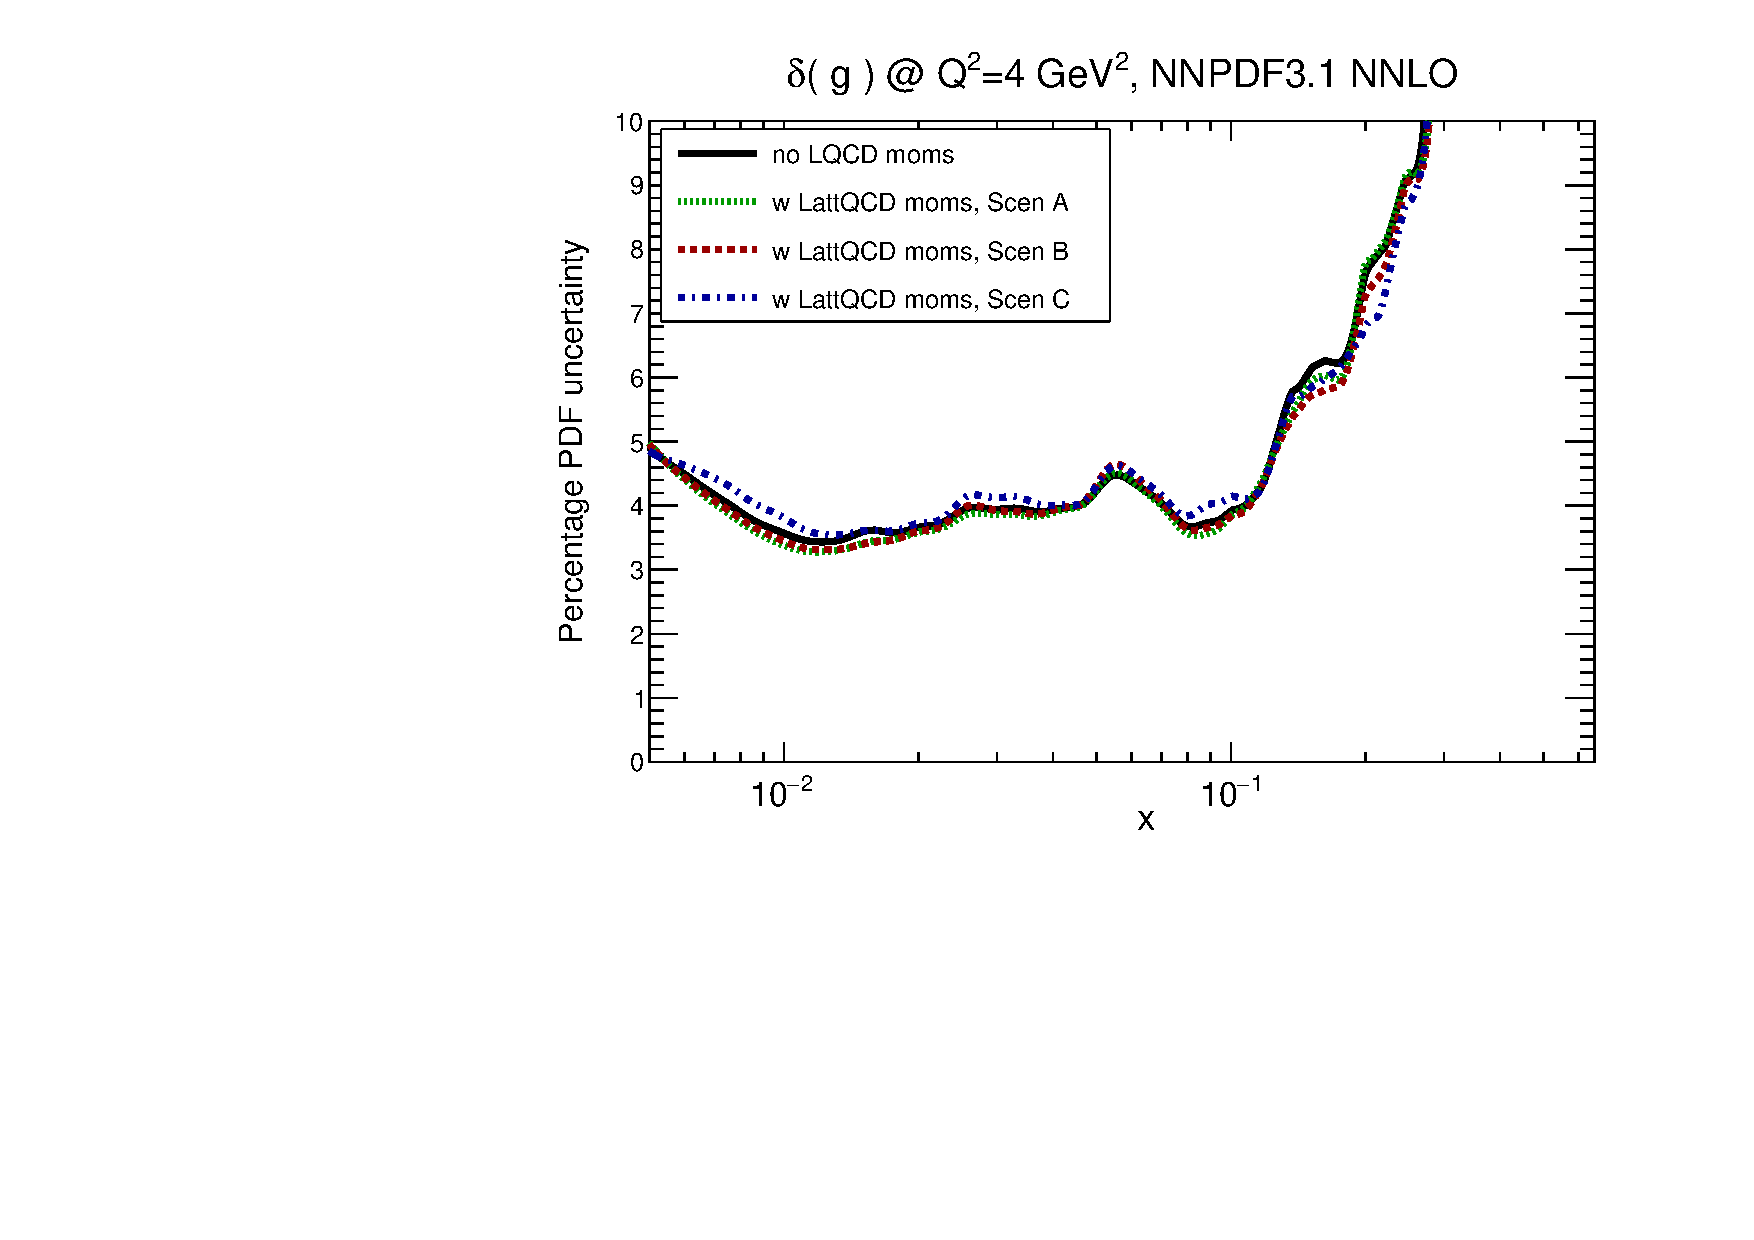
\includegraphics[scale=0.45]{plots/xg-unpol-lattice-relerr.pdf}
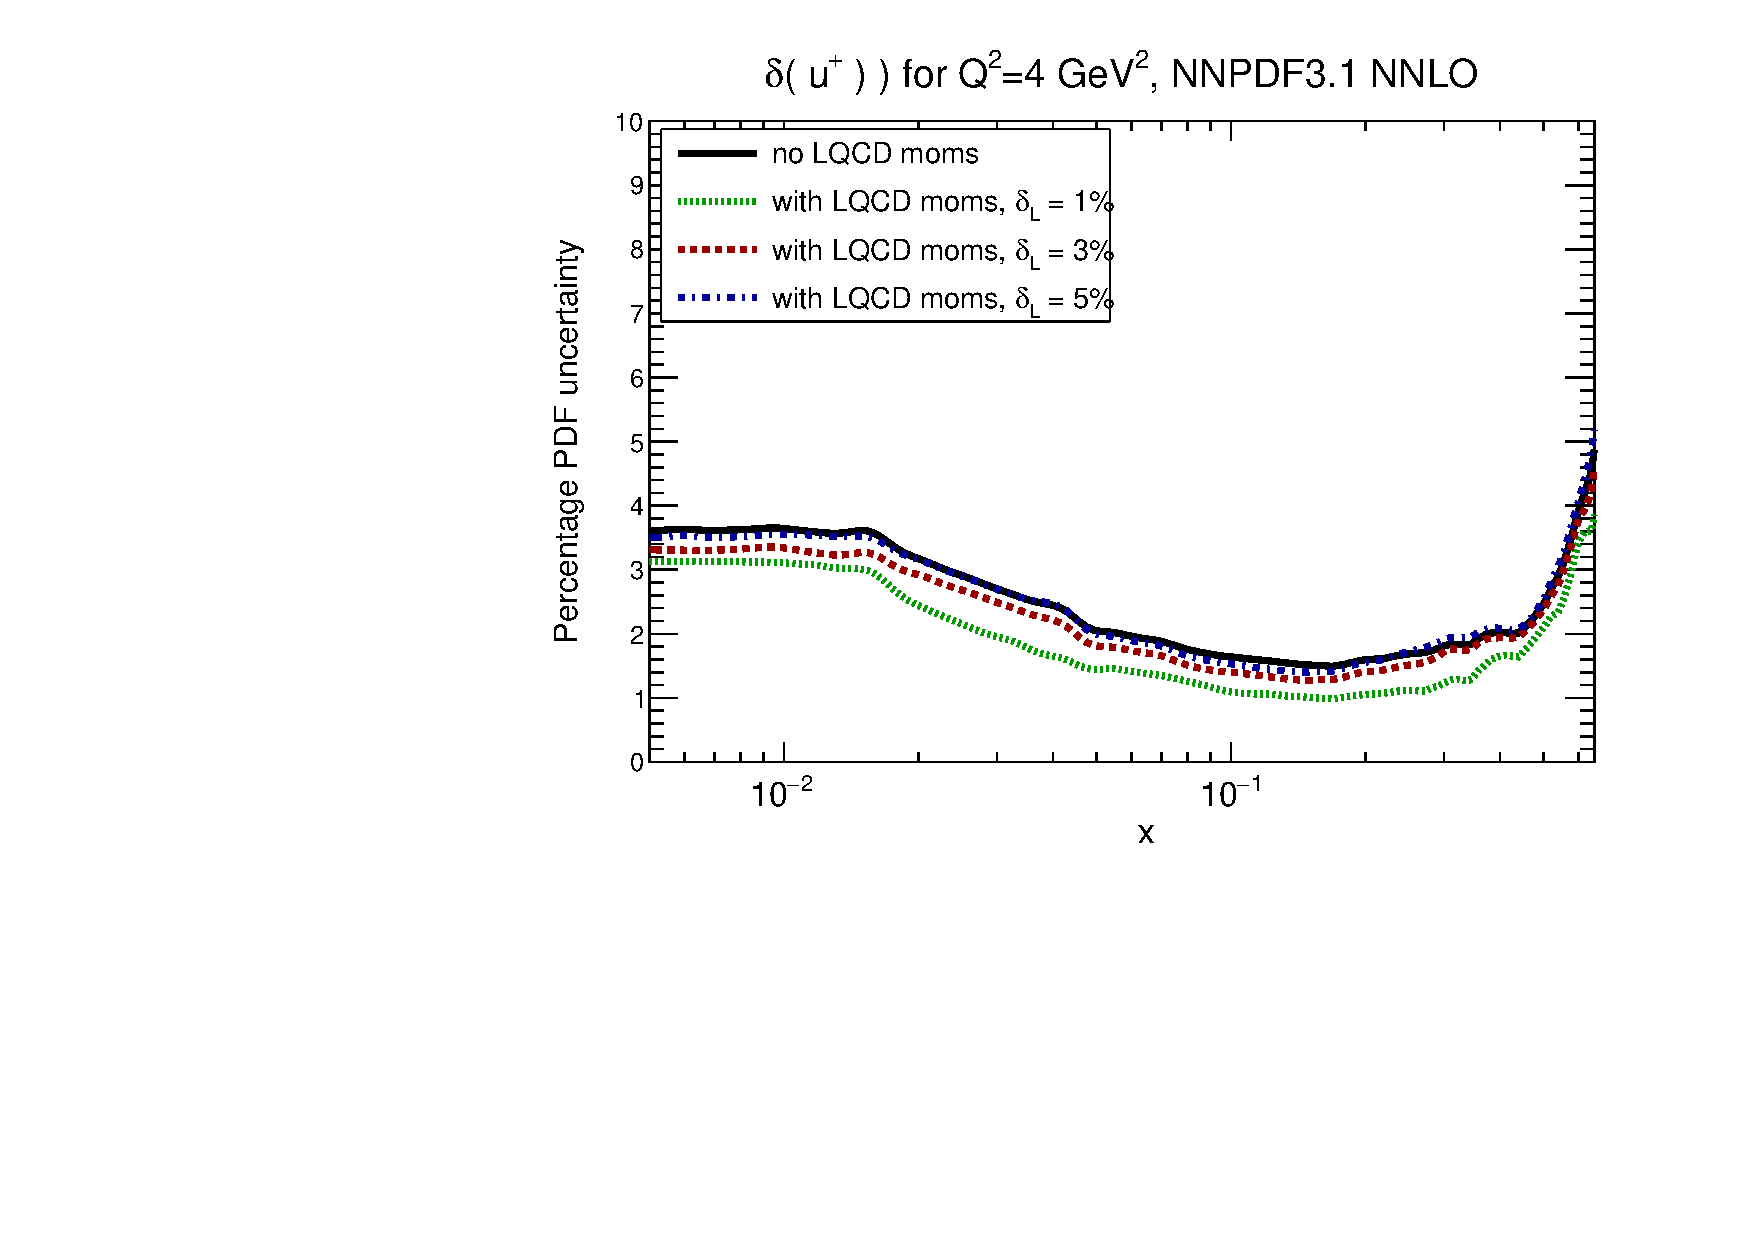
\includegraphics[scale=0.45]{plots/xup-unpol-lattice-relerr.pdf}
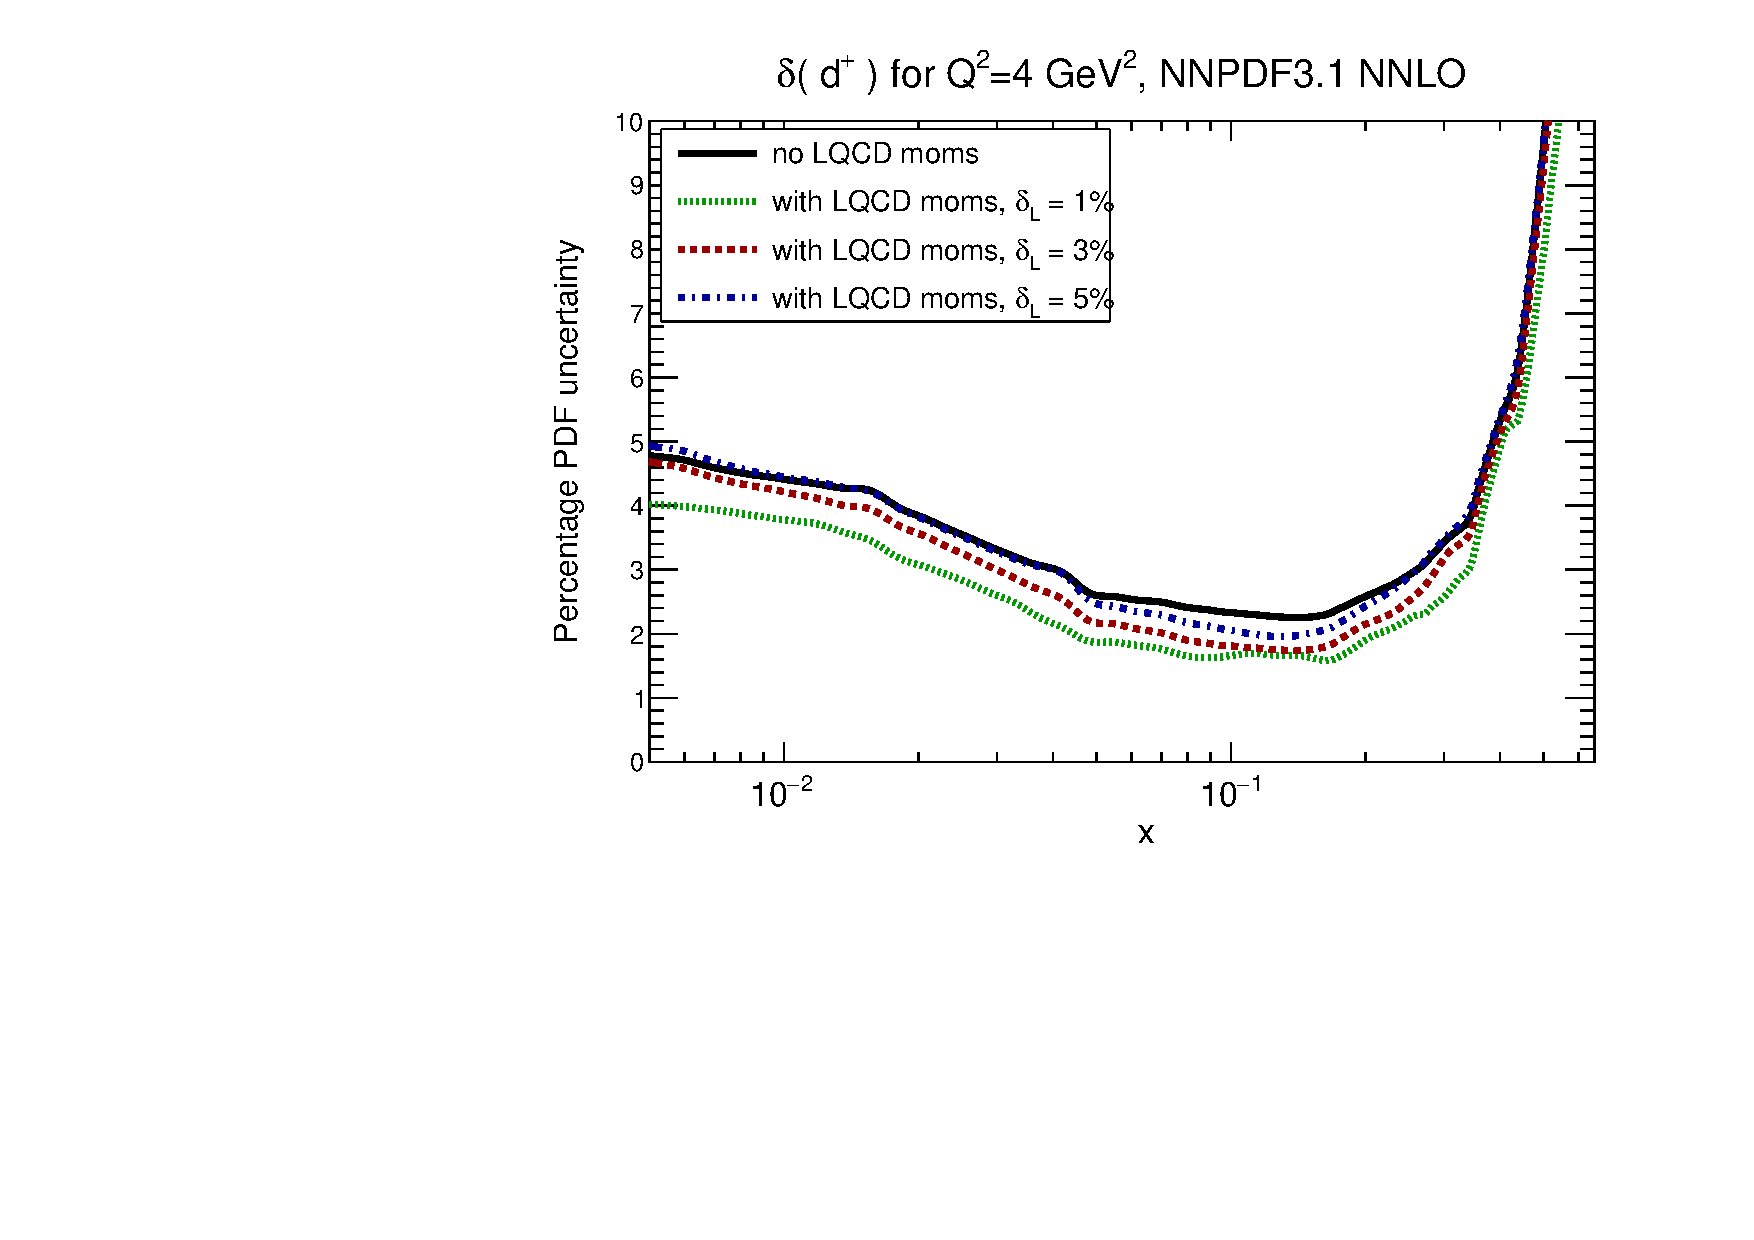
\includegraphics[scale=0.45]{plots/xdp-unpol-lattice-relerr.pdf}
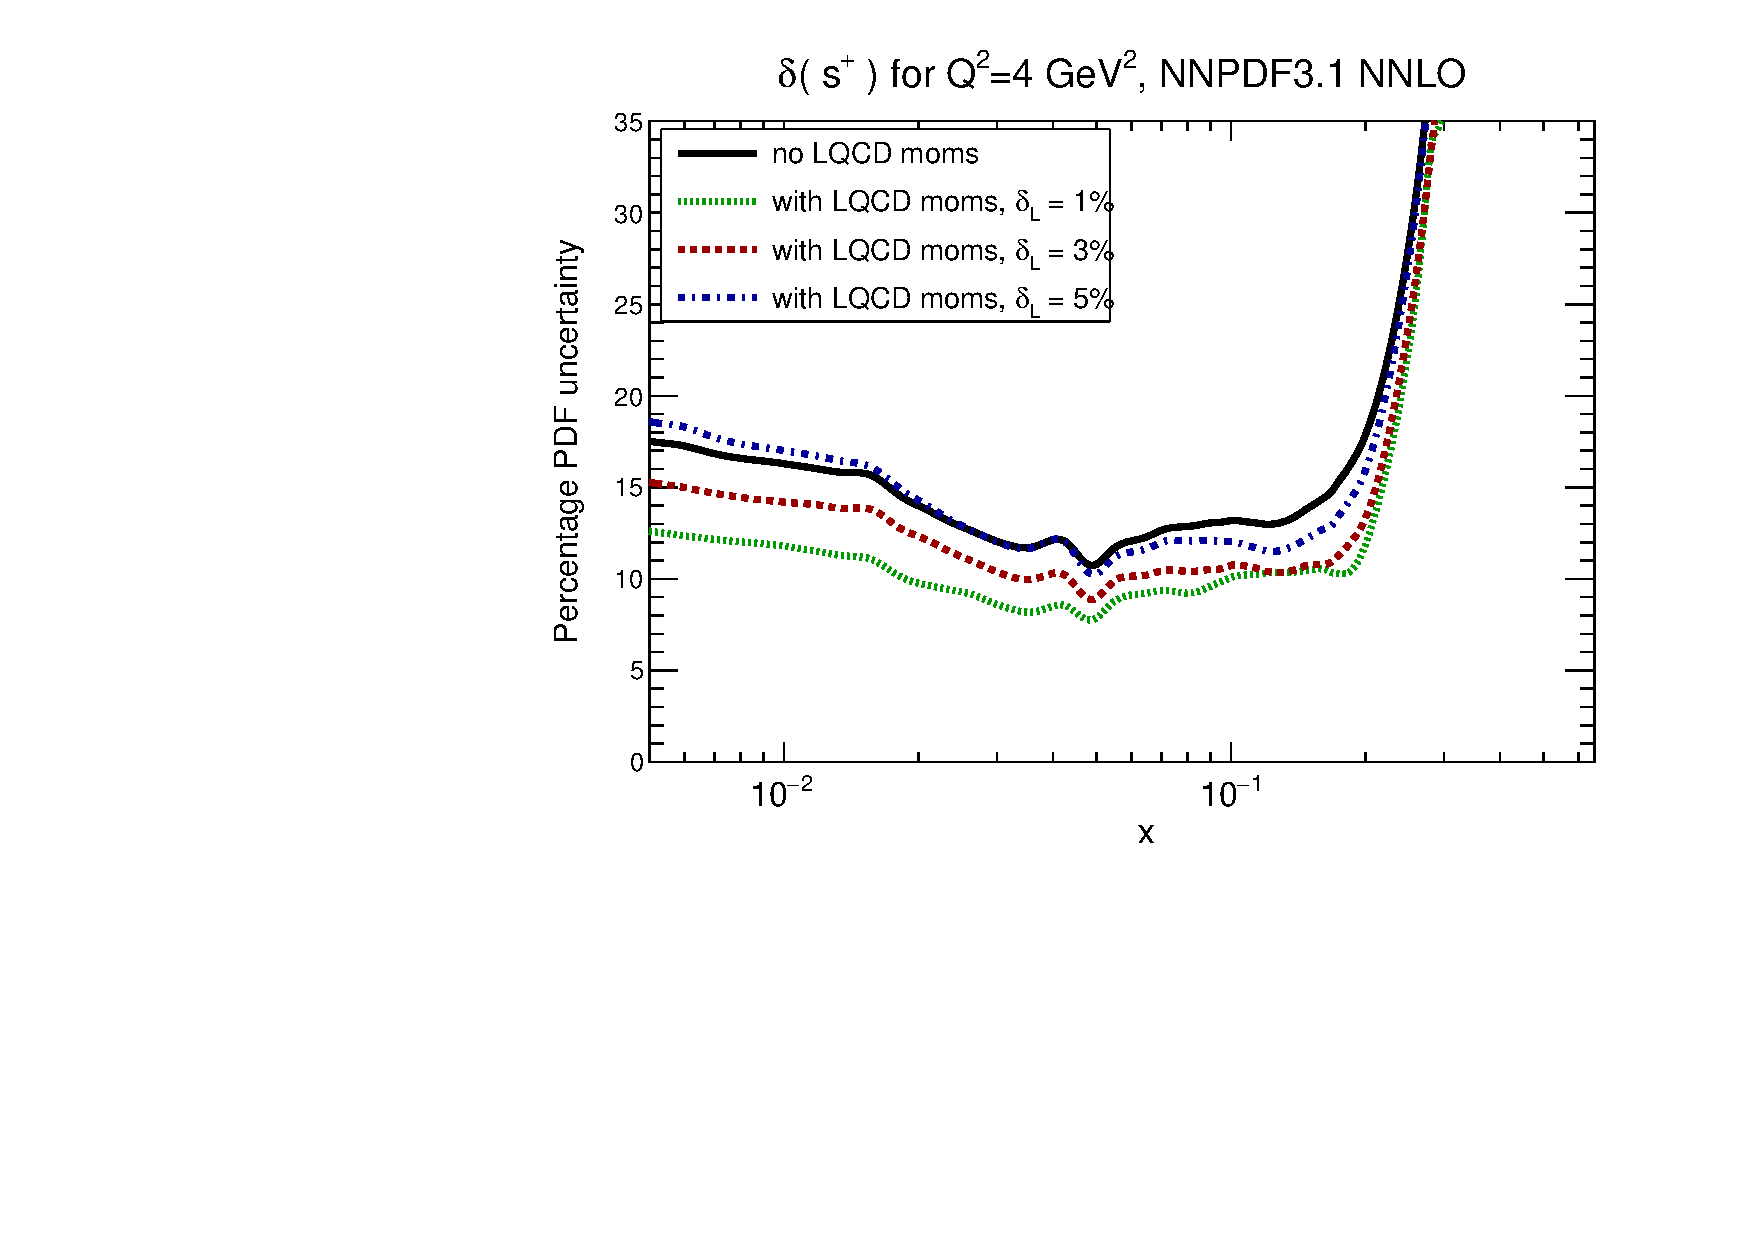
\includegraphics[scale=0.45]{plots/xsp-unpol-lattice-relerr.pdf}
\caption{\small The percentage PDF uncertainty in NNPDF3.1  
  for the gluon and the $u^+$, $d^+$ and $s^+$ quark PDFs at
  $Q^2=4$ GeV$^2$,
  compared to the results of including the five lattice
  QCD moments as pseudo-data points in the fit using the three
  different scenarios in  Table~\ref{tab:scenarios}.
  %
See text for more details.
}    
\label{fig:impactUnpol}
\end{figure}
%----------------------------------------------------------

The result that, at least with the specific moments that we have used
in this exercise, it will be challenging to reduce the
PDF uncertainties is also illustrated by the comparisons of 
 Fig.~\ref{fig:impactUnpol}, where we show
the percentage PDF uncertainties in NNPDF3.1  
for the gluon and the $u^+$, $d^+$ and $s^+$ quark PDFs in NNPDF3.1  
at $Q^2=4$ GeV$^2$,
compared to the corresponding results once
the lattice-QCD pseudo-data points of Table~\ref{tab:scenarios} have
been added by reweighting.
  %
In the case of the $u^+,d^+$ and $s^+$, we observe a slight reduction
of the PDF uncertainties, which is more marked as the move
from scenario A to C.
%
For instance, in the latter case the percentage PDF
uncertainty on $u^+$ ($d^+$ and $s^+$) at $x\simeq 0.1$
decreases from 1.8\% to 1.2\% (from 2.2\% to 1.7\% and from 13\% to 10\% respectively).
%
The PDF uncertainties of the gluon PDF, however,
are essentially unchanged even in the most optimistic scenario.

Focusing on the large-$x$ region, where the
impact of the PDF moments considered here
is expected to be more marked,
Fig.~\ref{fig:impactUnpollargex} we show a similar comparison
as in Fig.~\ref{fig:impactUnpol} but now showing the ratio of the
  PDF uncertainties in the fits based on the three scenarios
  as a ratio of the original
  PDF uncertainty of the NNPDF3.1   set, for the $d^+$
  and $s^+$ total quark PDFs.
  %
  This comparison illustrates better that the relative reduction
  of the PDF uncertainties upon the addition of the lattice-QCD
  pseudo-data is not completely flat, and that it exhibits some
  non-trivial structure.
  %
  Specifically we find that the constrains from the
  lattice-QCD computation of these PDF moments is more marked
  for $x\simeq 0.2$, and then decreasing for
  larger values of $x$.

%------------------------------------------------------
\begin{figure}[!t]
\centering
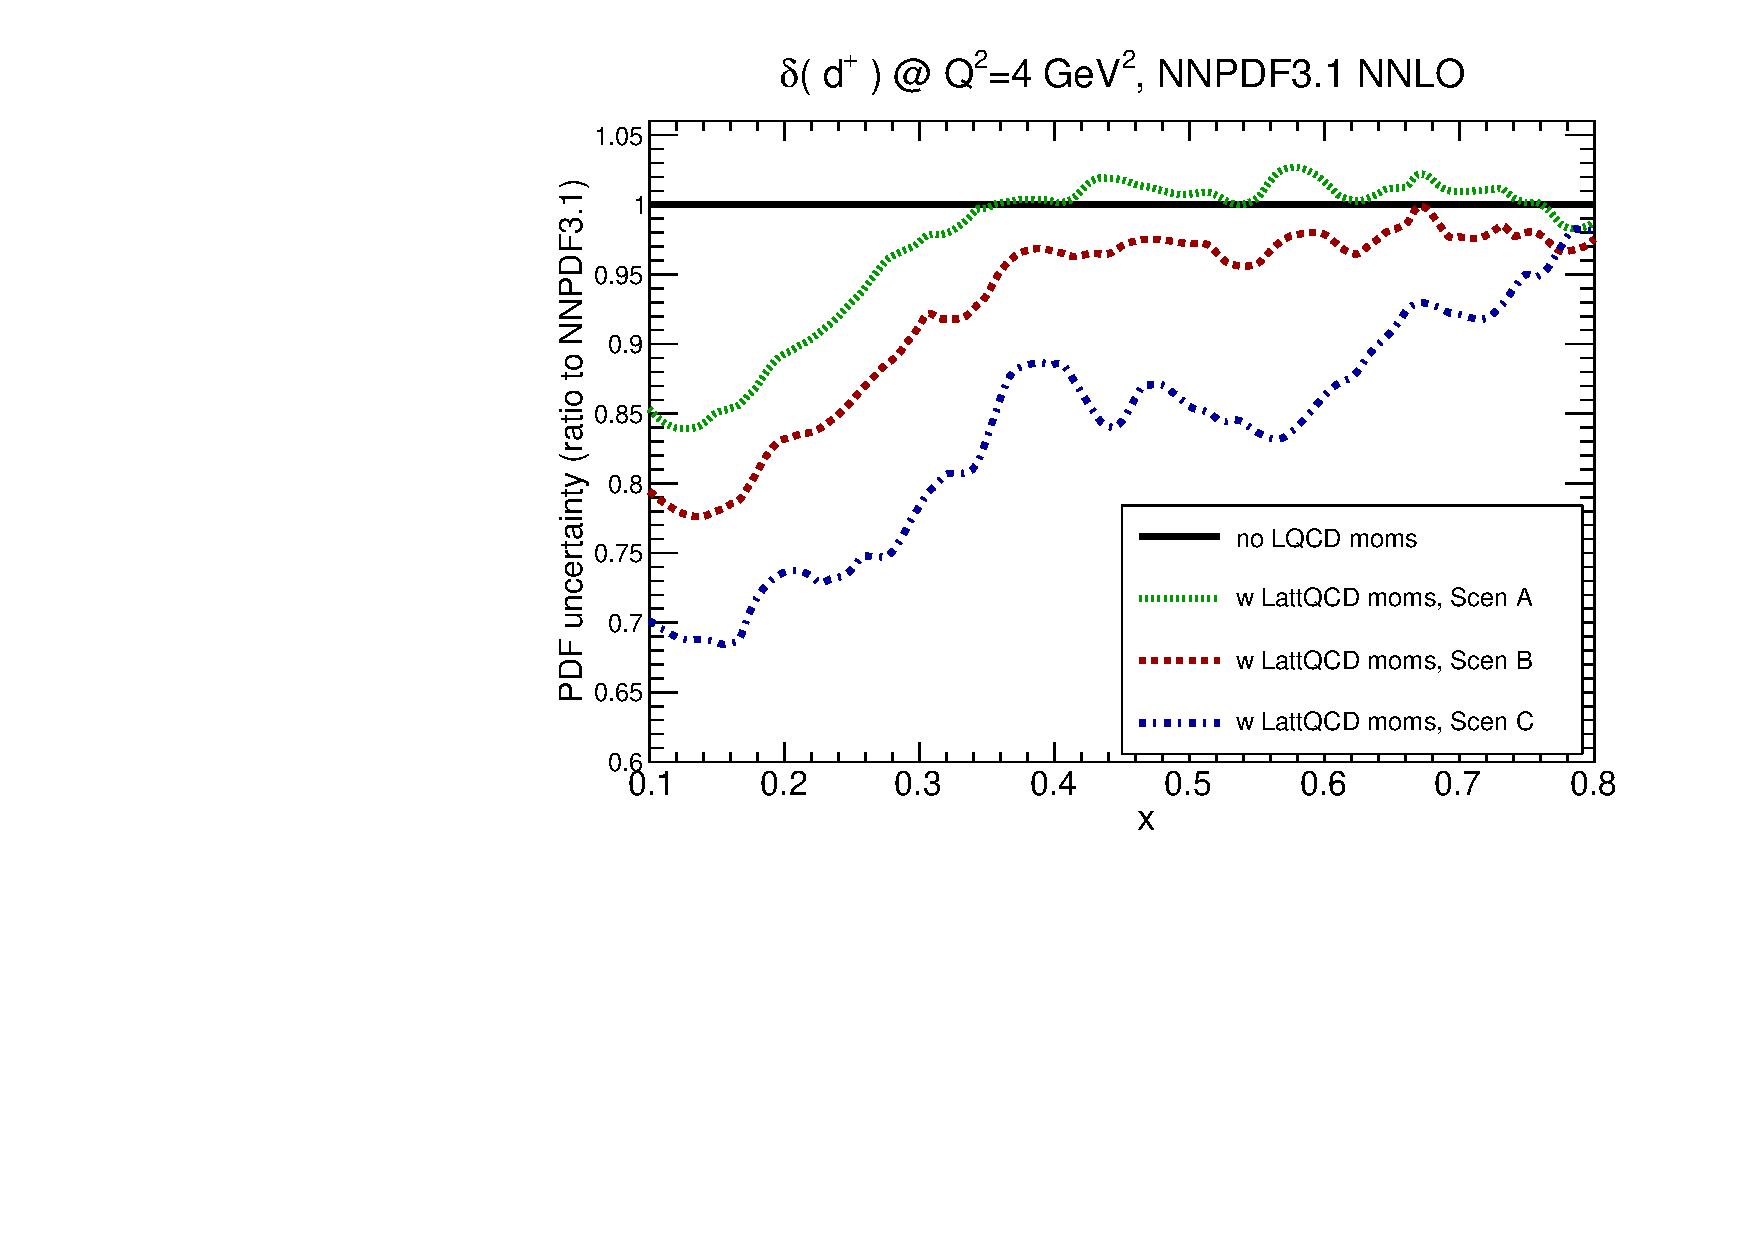
\includegraphics[scale=0.45]{plots/xdp-unpol-lattice-relerr-largex.pdf}
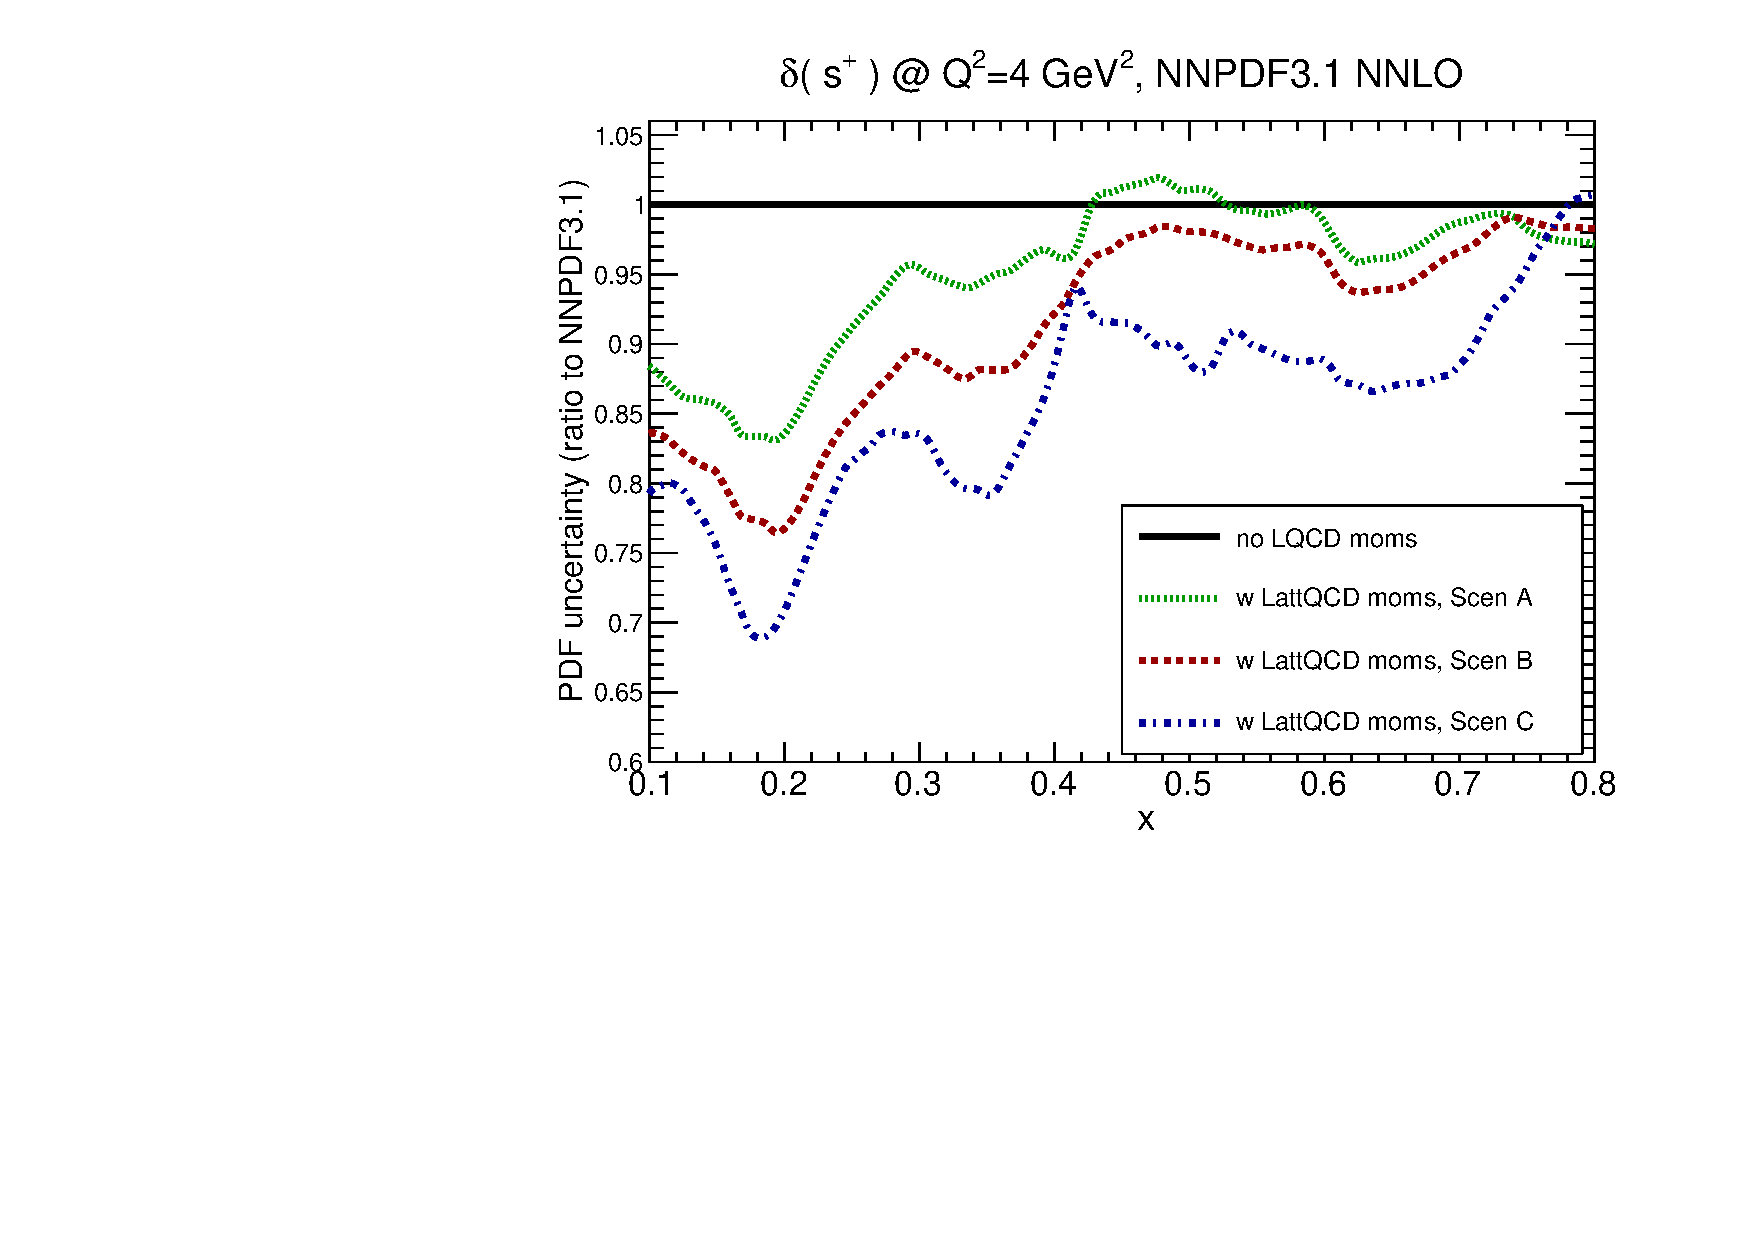
\includegraphics[scale=0.45]{plots/xsp-unpol-lattice-relerr-largex.pdf}
\caption{\small Same as Fig.~\ref{fig:impactUnpol}, now focusing
  on the large-$x$ region, and showing the ratio of the
  PDF uncertainties in the fits based on the three scenarios
  as a ratio of the original
  PDF uncertainty of the NNPDF3.1 set, for the $d^+$
  and $s^+$ total quark PDFs.
}    
\label{fig:impactUnpollargex}
\end{figure}
%----------------------------------------------------------

\paragraph{Impact on polarized global fits}
%
Now we turn to discuss the results of applying the
reweighting procedure to a representative polarized
global fit, specifically the NNPDFpol1.1 NLO set.
%
First of all, in Table~\ref{tab:polmomentsrw}
we list the values of the polarized PDF moments
  used as pseudo-data, as well as the corresponding results
  after the reweighting has been performed for the
three scenarios summarized in 
in Table~\ref{tab:scenarios}.
%
As in the unpolarized case, the PDF uncertainties quoted correspond in all cases to 68\%
CL intervals.
%
As we can see from this comparison, already in the first scenario
(which assumes lattice-QCD pseudo-data with similar uncertainties
as existing calculations) there is a marked impact on the
polarized PDF moments.
%
Specifically, for both $\la 1\ra_{\Delta u^+}$ and $\la 1\ra_{\Delta d^+}$
the PDF uncertainties are roughly halved, with the same
trend but less marked for $\la 1\ra_{\Delta s^+}$.
%
At this level, there is no impact for the non-singlet
combinations $\la 1\ra_{\Delta u^+ - \Delta d^+}$
and $\la x\ra_{\Delta u^--\Delta d^-}$.

%%%%%%%%%%%%%%%%%%%%%%%%%%%%%%%%%%%%%%%%%%%%%%%%%%%%%%%%
\begin{table}[t]
  \centering
  \renewcommand{\arraystretch}{1.4} 
\begin{tabular}{c||c||c|c|c}
  \hline &  Original  & Scen A  &  Scen B  & Scen C  \\
  \hline
  $\la 1\ra_{\Delta u^+}$    &  $+0.788\pm  0.079$   & $+0.798\pm  0.039$     &
  $+0.797\pm  0.023$ &   $+0.790\pm  0.009$ \\
  $\la 1\ra_{\Delta d^+}$   &  $-0.450 \pm 0.083$  &  $-0.450 \pm 0.042$  &
  $-0.456 \pm 0.026$    &  $-0.465 \pm 0.012$   \\
  $\la 1\ra_{\Delta s^+}$    &  $-0.124\pm   0.108 $  & $-0.120\pm   0.070 $  &
  $-0.121\pm   0.076 $    &   $-0.111\pm   0.029 $  \\
  $\la 1\ra_{\Delta u^+ - \Delta d^+}$  & $+1.250 \pm 0.024$   & $+1.250 \pm 0.022$  &
  $+1.253 \pm 0.016$ &    $+1.256 \pm 0.012$  \\
  $\la x\ra_{\Delta u^--\Delta d^-}$     & $+0.196 \pm 0.014$    & $+0.195 \pm 0.014$
  & $+0.196 \pm 0.016$     &  $+0.198 \pm 0.012$    \\
  \hline
\end{tabular}
\caption{\small Same as Table~\ref{tab:unpolmomentsrw}, now for
  the polarized PDF moments computed with NNPDFpol1.1.
  %
  The corresponding impact at the PDF level is shown in
  Fig.~\ref{fig:impactPol}.
\label{tab:polmomentsrw}
}
\end{table}
%%%%%%%%%%%%%%%%%%%%%%%%%%%%%%%%%%%%%%%%%%%%%%%%%%%%%%%%

As we further decrease the assumed uncertainties in the lattice-QCD pseudo-data
for the PDF moments, we observe a consequent reduction of the uncertainties
in the global fit.
%
In the most optimistic scenario C, we find that for both
$\la 1\ra_{\Delta u^+}$ and $\la 1\ra_{\Delta d^+}$ there is an uncertainty
reduction by about an order of magnitude as compared to the current values,
and about a factor 5 for $\la 1\ra_{\Delta s^+}$.
%
Therefore, we demonstrate that future lattice-QCD calculations of
polarized PDF moments can potentially lead to a much more
precise understanding of the spin structure of the proton.
%
The other quark combinations exhibit less sensitivity to the inclusion
of the PDF moments in the global fit, given that to begin with
they are already quite well constrained by available experimental
data.
%
Specifically, the PDF uncertainties for  $\la 1\ra_{\Delta u^+ - \Delta d^+}$
are reduced by a factor 2 in this quite optimistic scenario, while
those of $\la x\ra_{\Delta u^--\Delta d^-}$ are essentially unaffected even
in this case.

Next we move to illustrate the impact of the lattice-QCD pseudo-data
on the polarized PDFs themselves, rather than on their
moments.
%
With this motivation,
in Fig.~\ref{fig:impactPol} we present a 
similar comparison as that of Fig.~\ref{fig:impactUnpol}, now
  showing the absolute PDF uncertainties of the NNPDFpol1.1 fit,
  compared to the corresponding results once the lattice pseudo-data
  on polarized moments in included in the analysis by means of the
  reweighting.
  %
  The reason to show absolute rather than relative uncertainties
  is that, unlike unpolarized PDFs, polarized PDFs often exhibit nodes
  (in particular for strangeness and the gluon) and in the nearby regions
  the concept of relative uncertainty becomes ill-defined.
  
%-------------------------------------------------------------------
\begin{figure}[!t]
\centering
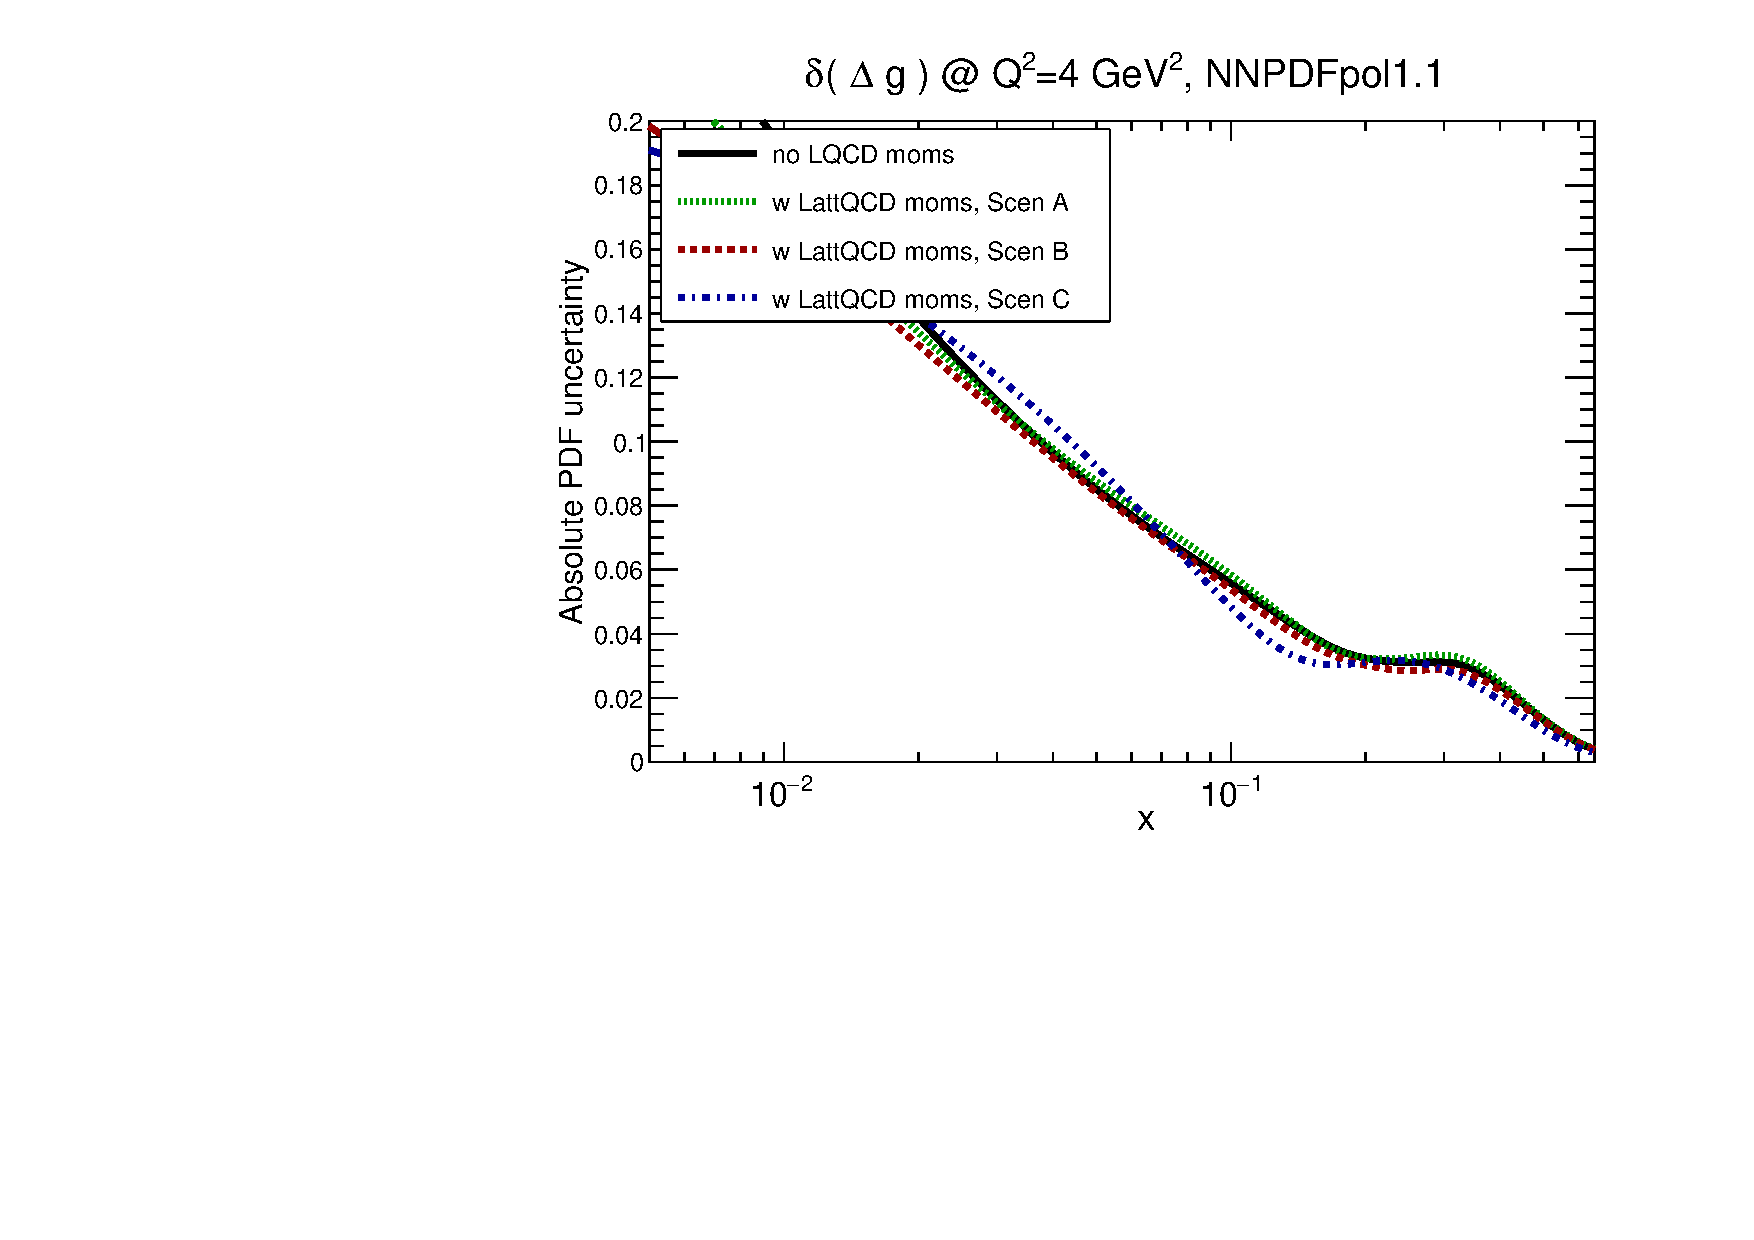
\includegraphics[scale=0.45]{plots/xg-pol-lattice-relerr.pdf}
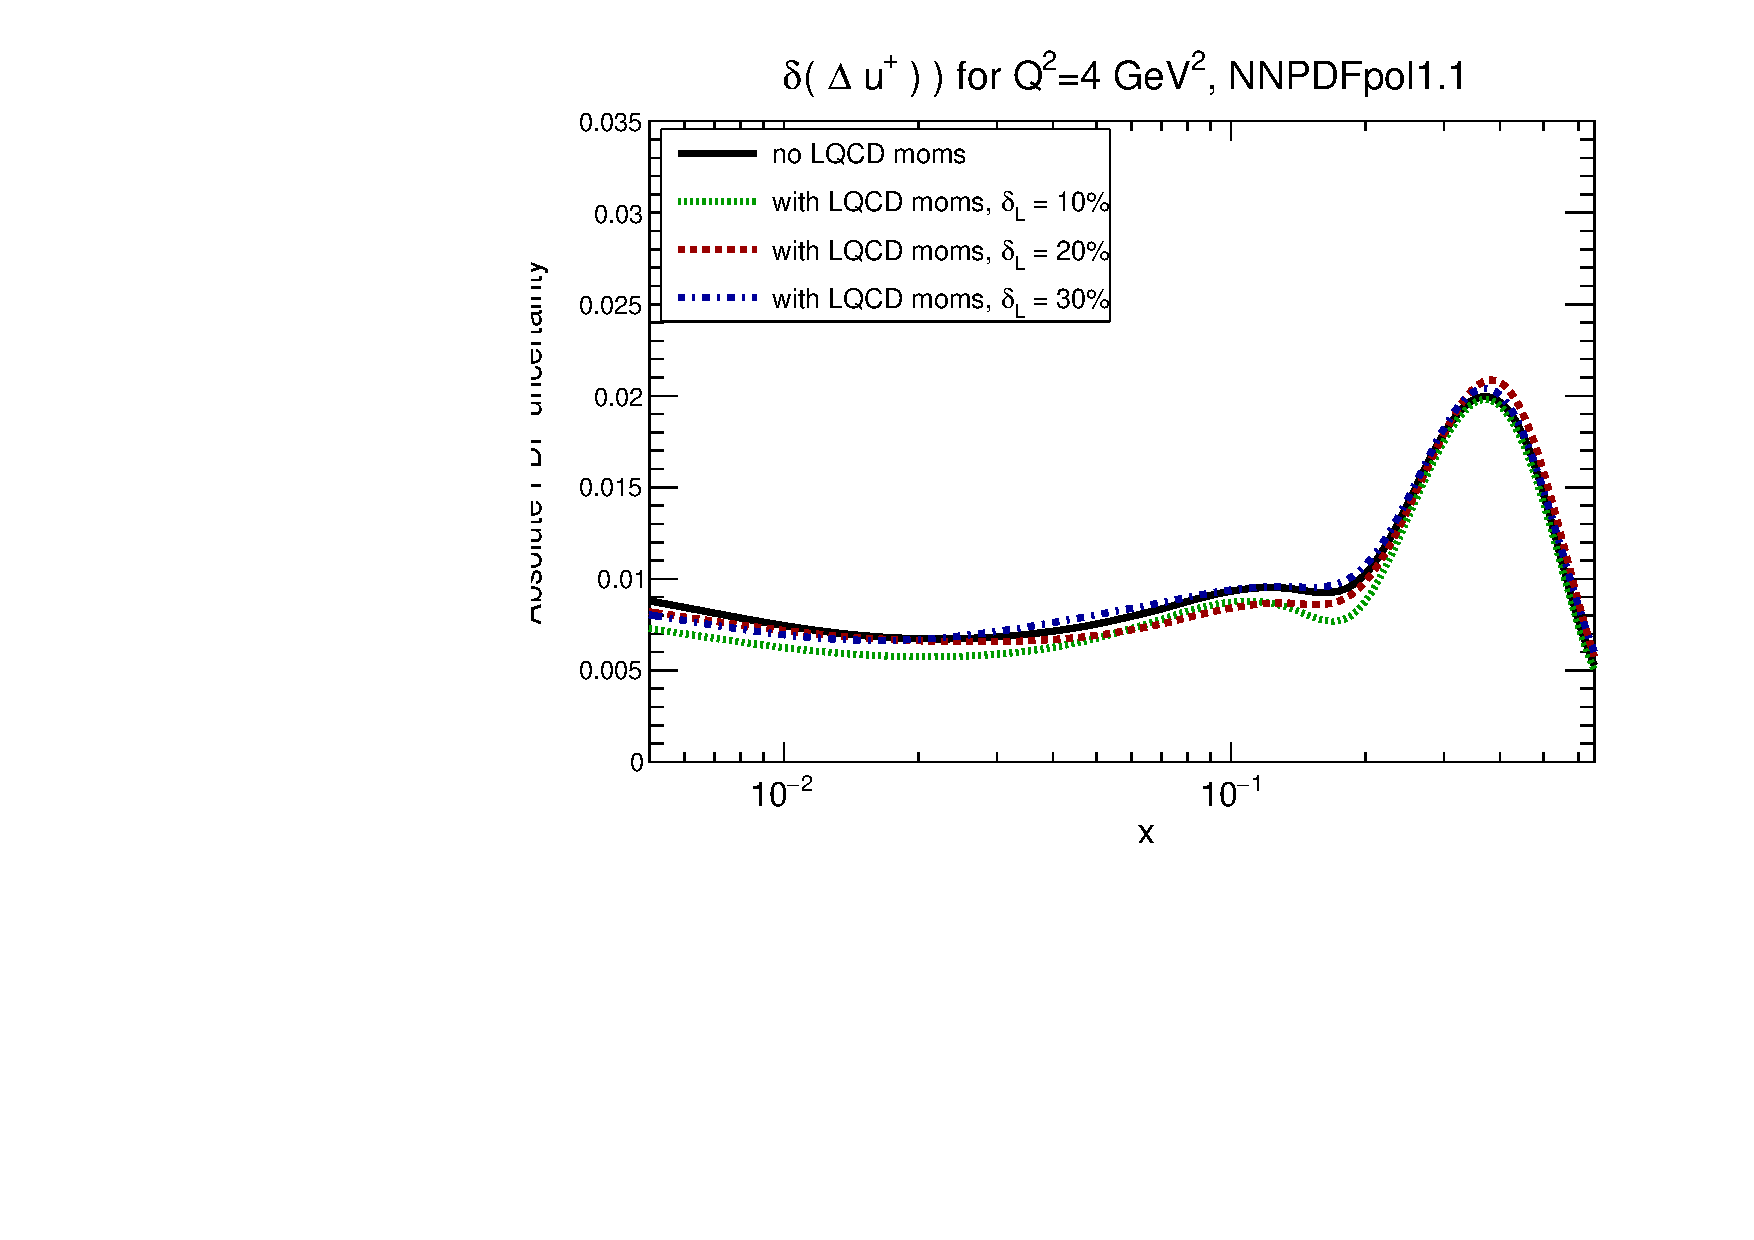
\includegraphics[scale=0.45]{plots/xup-pol-lattice-relerr.pdf}
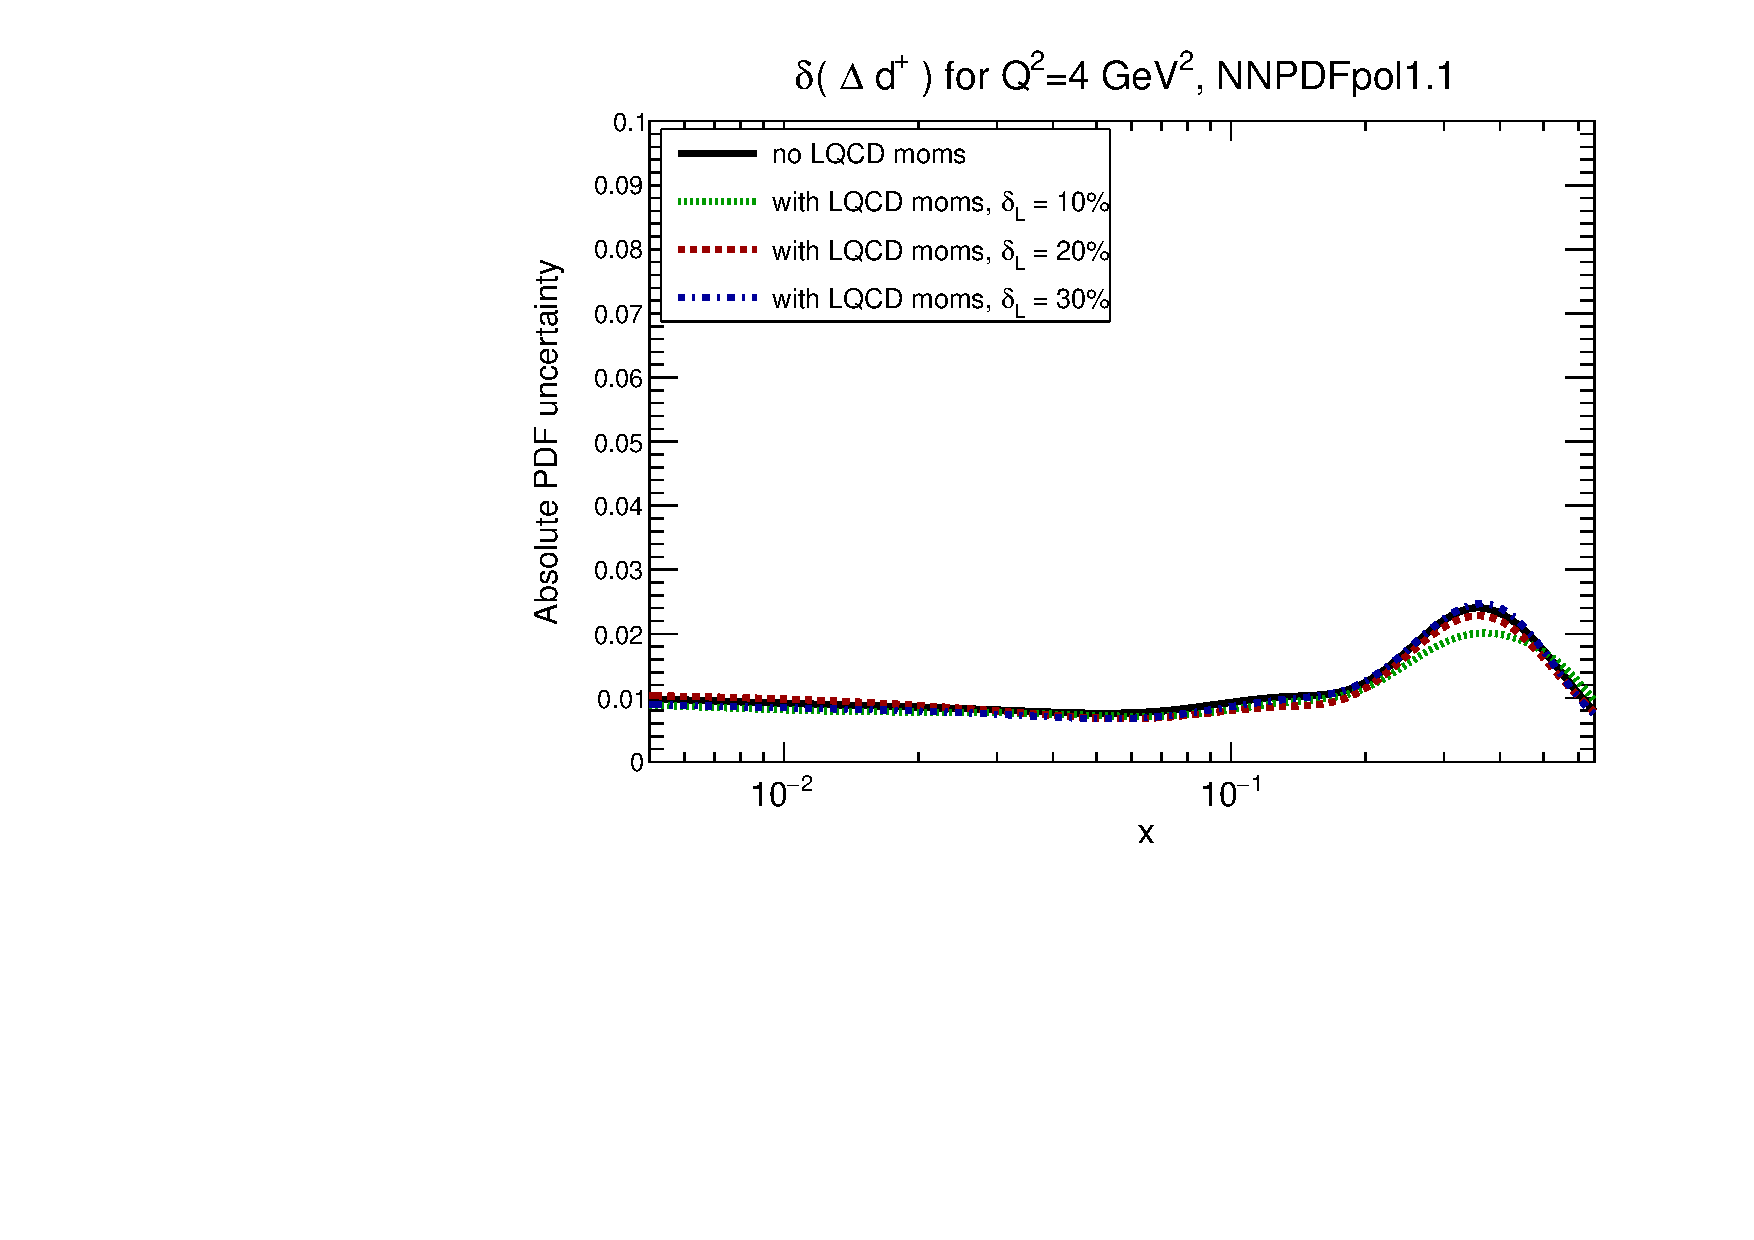
\includegraphics[scale=0.45]{plots/xdp-pol-lattice-relerr.pdf}
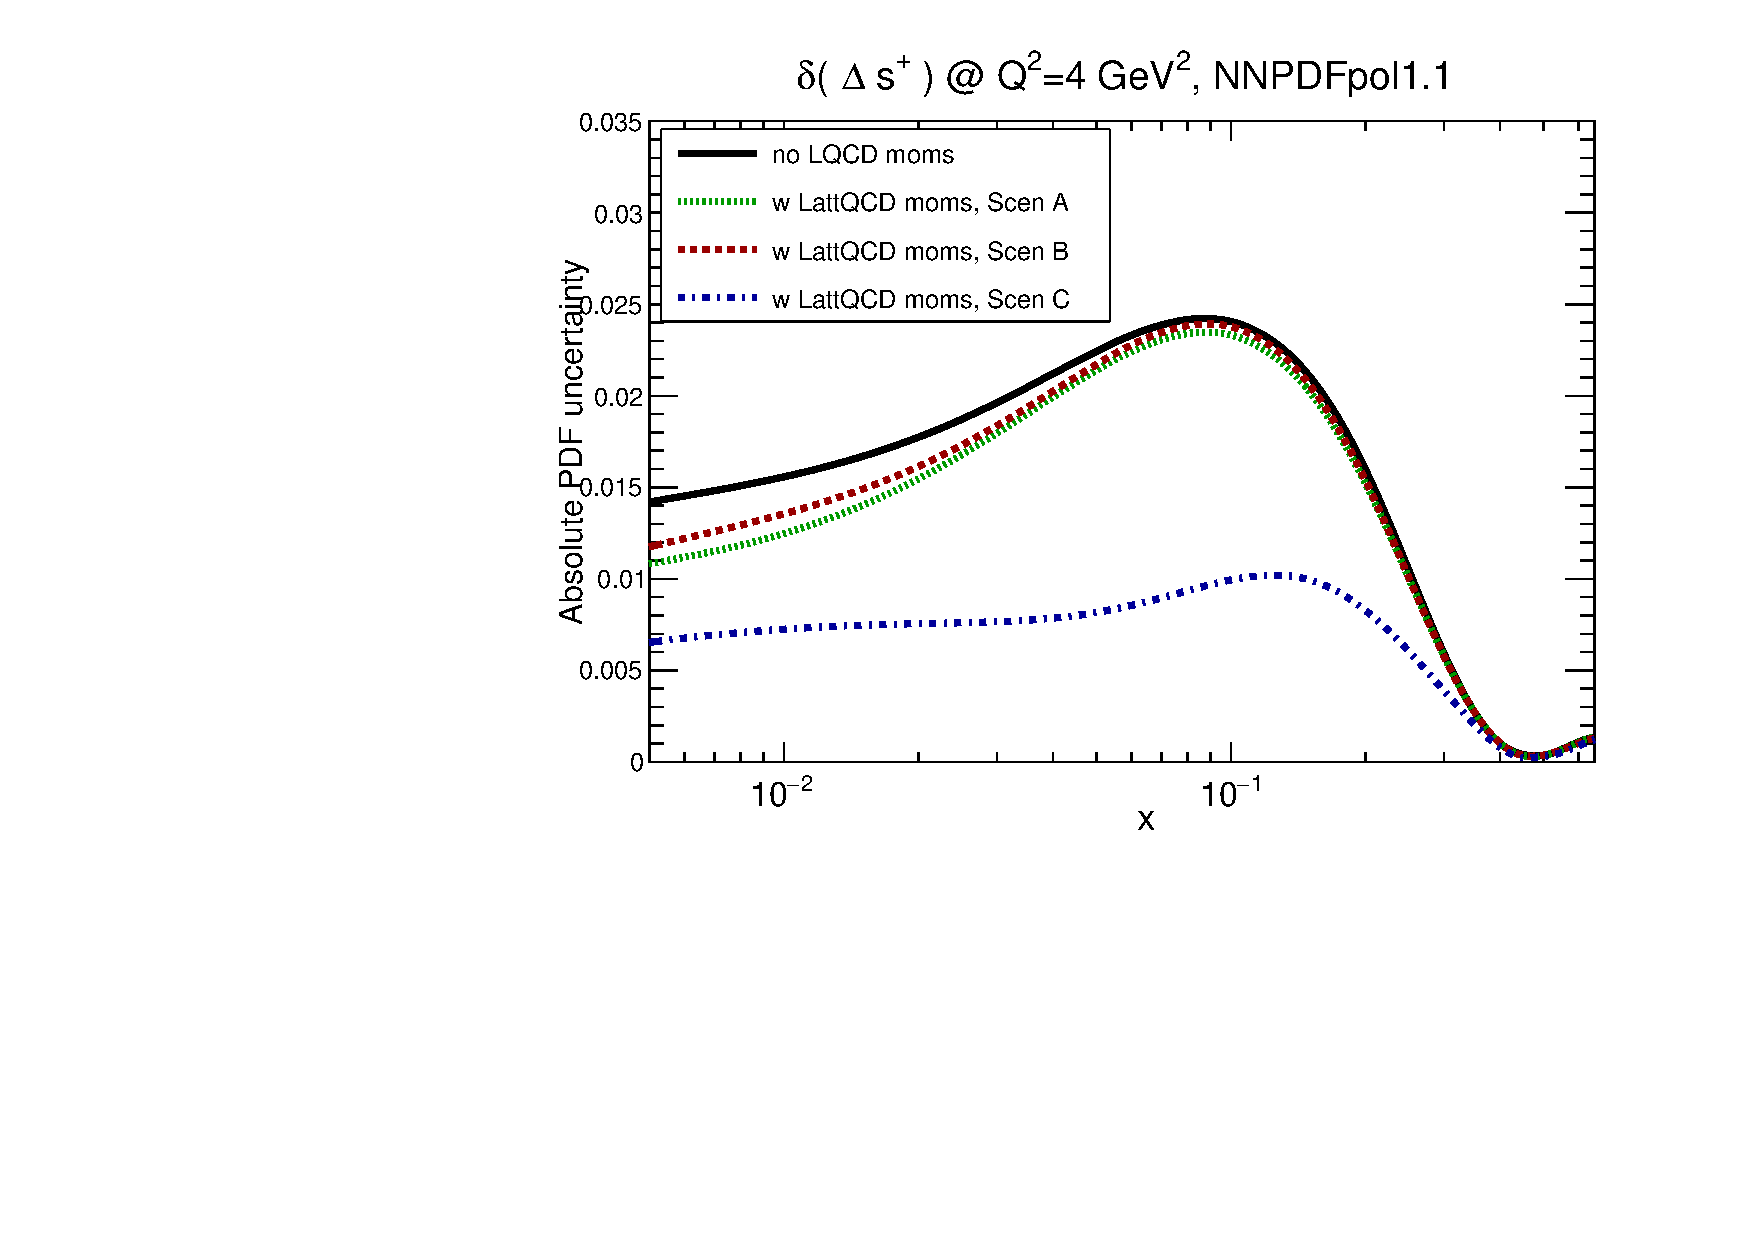
\includegraphics[scale=0.45]{plots/xsp-pol-lattice-relerr.pdf}
\caption{\small Same as Fig.~\ref{fig:impactUnpol}, now
  showing the absolute PDF uncertainties of the NNPDFpol1.1 fit
   $Q^2=4$ GeV$^2$,
  compared to the corresponding results once the lattice pseudo-data
  on polarized moments in included in the analysis via
  reweighting.
}    
\label{fig:impactPol}
\end{figure}
%---------------------------------------------------------------------

From Fig.~\ref{fig:impactPol} we find that for scenarios
A and B there only a very moderate reduction (or even a slight increase)
of the PDF uncertainties, seemingly at odds with the results
for their moments in Table~\ref{tab:polmomentsrw}.
%
The reason is that the first PDF moments alone provide only limited
information on the shape of the PDFs itself, and therefore in some
cases one will find a large error reduction on the moments (since these
are the fitted quantified) than on the PDFs themselves (which are
only directly constrained).
%
On the other hand, once the lattice-QCD pseudo-data uncertainties
decrease beyond a certain level, the start to impact the PDF shape
as well, as we can see from the results of scenario C.
%
In that case we find that the PDF uncertainties can decreases by up to a factor
2 (3) for $\Delta d^+(x,Q)$ ($\Delta s^+(x,Q)$).
%
Interestingly, we see that the relative reduction of PDF uncertainties is more
or less constant along the whole range of $x$, consistent with the fact that
the lattice-QCD pseudo-data is only sensitive to the total integral
of the $x$ distribution.



% PDF moment analysis using Hessian profiling 
\subsubsection{Hessian profiling analysis}
\label{sec:hessianprofiling}

% Results of the Hessian profiling using HERAPDF2.0 as input.


We can also use a profiling method with Hessian PDF uncertainty sets  
to estimate the effect of including Lattice data into the fit. 
This is similar to the  reweighting method used with the Monte Carlo PDFs (NNPDF3.0) 
in Sec.\ref{subsec:upolfits},
and the details of our approach can be found in~\cite{Paukkunen:2014zia,Camarda:2015zba}.
%
We choose the HERAPDFs as a representative set of Hessian PDFs, and 
we have used the same Lattice data on moments to estimate the impact
on the HERAPDF2.0 unpolarized Hessian PDFs~\cite{Abramowicz:2015mha}. 
%
An additional advantage of the HERAPDFs is that they use
$\Delta\chi^2=1$ for defining the Hessian error PDFs which ensures a
one to one correspondence of the profiling and reweighting methods.

%============

In case of Hessian PDF sets, the Hessian profiling method
can be used to both check the compatibility of new data on a given PDF set,
and also  estimate the impact these data will have on the PDFs. 
In the following we describe essential components of the profiling method, 
and will assume  that the considered Hessian PDF set is using tolerance of $\Delta\chi^2=1$ 
which corresponds to 68\%~CL uncertainties.



%INTRO
The central values of the considered moments are obtained using the central PDFs and the corresponding
errors are calculated according to:
\begin{equation}
\delta\mathcal{F}_i = \frac{1}{2} \sqrt{\sum_{k}\left(\mathcal{F}_i(f_k^+)-\mathcal{F}_i(f_k^-)\right)^2},
\quad i=1,\ldots,N_{\rm mom}
\end{equation}
where $k$ numbers the error PDFs.
%
In the profiling method we consider a $\chi^2$ function in which the $\chi^2$ of the new
data has been added to the initial $\chi^2$:
\begin{equation}
\label{eq:newchi2}
\chi^2_{\text{new}} = \chi_0^2 + \sum_{k}^{N_{\text{eig}}} z_k^2
                    + \sum_{i=1}^{N_{\text{data}}}
                      \frac{\lp \mathcal{F}_i - \mathcal{F}_i^{\rm(exp)}\rp^2}
                           {\lp\delta\mathcal{F}_i^{\rm(exp)}\rp^2}
\end{equation}
where $\chi^2_0$ is the value of the $\chi^2$ function in the minimum of the initial PDF set,
$z_k$ are parameters diagonalizing the Hessian matrix of the initial PDF set,
$N_{\text{eig}}$ is the dimension of the eigenvector space in which initial Hessian errors are defined
(half of the number of error PDFs), $\mathcal{F}_i^{\rm(exp)}$ is the new data,
and $\mathcal{F}_i$ the corresponding theory prediction.

In the spirit of the Hessian method the new theory predictions $\mathcal{F}_i$ can be expanded
using a linear approximation:
\begin{equation}
\mathcal{F}_i \simeq \mathcal{F}_i[S_0] + \sum_k \frac{\partial\mathcal{F}_i[S]}{\partial z_k}\bigg|_{S=S_0} z_k \quad
              \simeq \mathcal{F}_i[S_0] + \sum_k D_{ik} w_k \ ,
\end{equation}
where $S_0$ represents central PDF and $D_{ik}=\frac{1}{2}(\mathcal{F}_i[S_k^+]-\mathcal{F}_i[S_k^-])$;
here the  derivative has been approximated by a finite difference of the 
Hessian PDF error sets $S_k^{\pm}$.
%
The new $\chi^2$ of Eq.~\eqref{eq:newchi2} can now be minimized with respect to the parameters $w_k$,
which results in:
\begin{equation}
\boldsymbol{\vec{w}_{\text{{\bf min}}}} = \boldsymbol{-B^{-1}} \boldsymbol{\vec{a}},
\end{equation}
with
\begin{equation}
%\begin{split}
B_{kn} = \sum_i \frac{D_{ik}D_{in}}{\lp\delta\mathcal{F}_i^{\rm(exp)}\rp^2} + \delta_{kn},
%\\
\qquad
\qquad
a_k = \sum_i \frac{D_{ik}(\mathcal{F}_i[S_0] - \mathcal{F}_i^{\rm(exp)})}{\lp\delta\mathcal{F}_i^{\rm(exp)}\rp^2} \ . 
%\end{split}
\end{equation}
%
The components of the solution $\boldsymbol{\vec{w}_{\text{{\bf min}}}}$ define a new set
of PDFs representing a global minimum after including the new data:
\begin{equation}
f_{\text{new}} = f_{S_0} + \sum_{k=1}^{N_{\text{eig}}} \frac{f_{S_k^+}-f_{S_k^-}}{2} w_k^{\text{min}} \ .
\end{equation}
At the same time $\boldsymbol{\vec{w}_{\text{{\bf min}}}}$ also  defines  a penalty term 
\begin{equation}
P = \sum_{k=1}^{N_{\text{eig}}} \lp w_k^{\text{min}} \rp^2
\end{equation}
which can be used to estimate whether the new data is consistent with the initial set of PDFs;
a penalty of $P\ll1$ means that the new data is consistent.
%
Finally, a set of new error PDFs can be also defined; in this case matrix $B_{kn}$ plays the role of
the Hessian matrix from which the PDF errors can be obtained. 




%======================================================================
%CONCLUSION
%
We have performed this study assuming the same 3 scenarios for the errors of the Lattice data,
{\it cf.,}~Table~\ref{tab:scenarios}. 
The study was performed using the xFitter program~\cite{Alekhin:2014irh}.
%
The results of the profiling are shown in Table~\ref{tab:unpolmomentsProf} where the uncertainties
of the considered moments are displayed for the case of the initial HERAPDF2.0 PDF and after including the Lattice
moments data in the three scenarios.
%
%
Additionally, in Fig.~\ref{fig:pdfsProf}, we show the impact of the Lattice data on the PDFs by
comparing the relative errors of the PDFs in scenarios A, B and C with initial HERAPDF2.0 errors.

%%%%%%%%%%%%%%%%%%%%%%%%%%%%%%%%%%%%%%%%%%%%%%%%%%%%%%%%
\begin{table}[h]
  \centering
  \renewcommand{\arraystretch}{1.3} 
\begin{tabular}{c||c|c|c|c}
  \hline &  Original  & Scen A  &  Scen B  &  Scen C  \\
  \hline
  \hline
  $\la x\ra_{u^+}$     &  $0.3720\pm 0.0036$  &  $0.3720\pm 0.0030$  &  $0.3720\pm 0.0027$  &  $0.3720\pm 0.0020$ \\
  $\la x\ra_{d^+}$     &  $0.1845\pm 0.0053$  &  $0.1845\pm 0.0028$  &  $0.1845\pm 0.0023$  &  $0.1845\pm 0.0015$ \\
  $\la x\ra_{s^+}$     &  $0.0346\pm 0.0037$  &  $0.0346\pm 0.0015$  &  $0.0346\pm 0.0012$  &  $0.0346\pm 0.0009$ \\
  $\la x\ra_{g}$       &  $0.4006\pm 0.0078$  &  $0.4006\pm 0.0042$  &  $0.4006\pm 0.0035$  &  $0.4006\pm 0.0024$ \\
  $\la x\ra_{u^+-d^+}$ &  $0.1875\pm 0.0074$  &  $0.1875\pm 0.0045$  &  $0.1875\pm 0.0039$  &  $0.1875\pm 0.0027$ \\
  \hline
\end{tabular}
\caption{\small Values of the unpolarized PDF moments
  used as pseudo-data, as well as the corresponding results
  after the profiling  for the
three scenarios summarized in Table~\ref{tab:scenarios}.
%
The HERAPDF2.0 PDFs were used, and the PDF uncertainties quoted correspond in all cases to 68\%~CL intervals.
\label{tab:unpolmomentsProf}
}
\end{table}
%%%%%%%%%%%%%%%%%%%%%%%%%%%%%%%%%%%%%%%%%%%%%%%%%%%%%%%%



%%%%%%%%%%%%%%%%%%%%%%%%%%%%%%%%%%%%%%%%%%%%%%%%%%%%%%%%
\begin{figure}[!t]
\centering
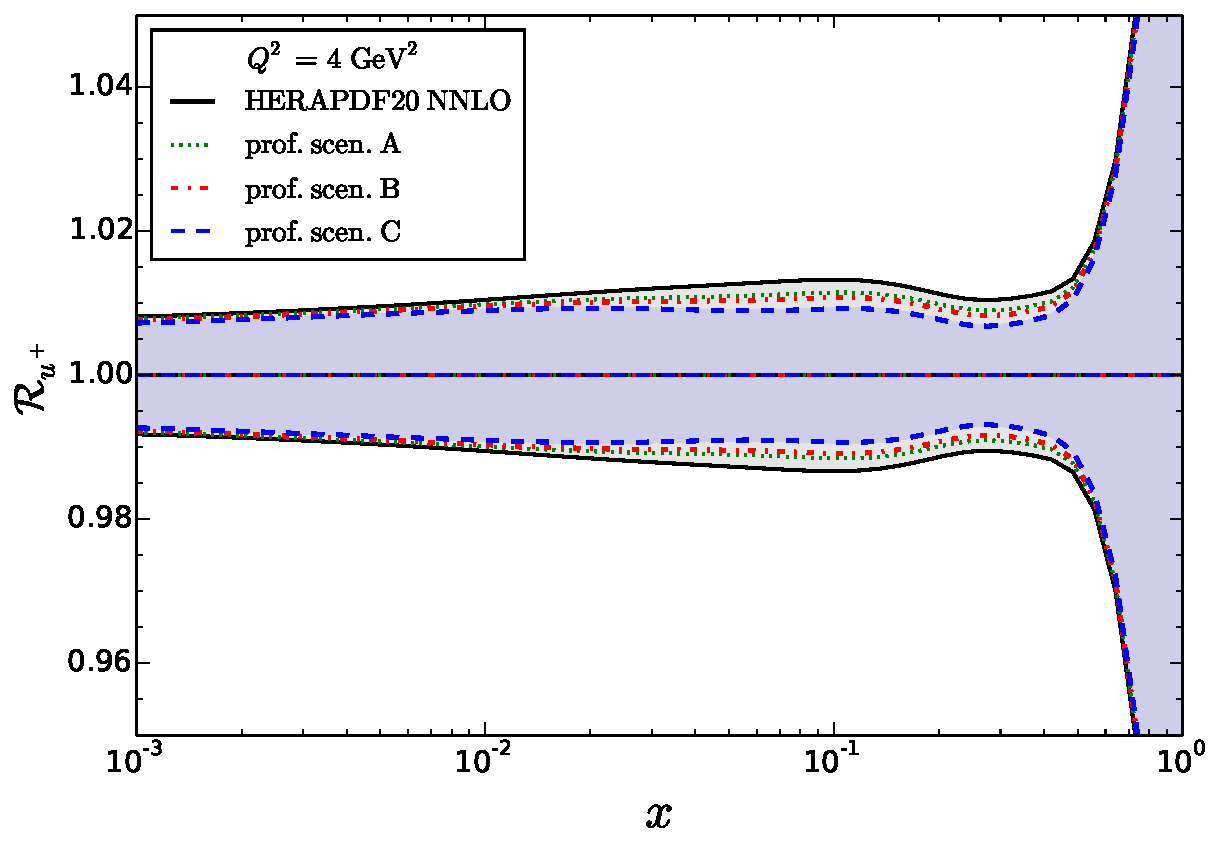
\includegraphics[width=0.45\textwidth]{plots/ratio_uPubar_Q2.pdf}
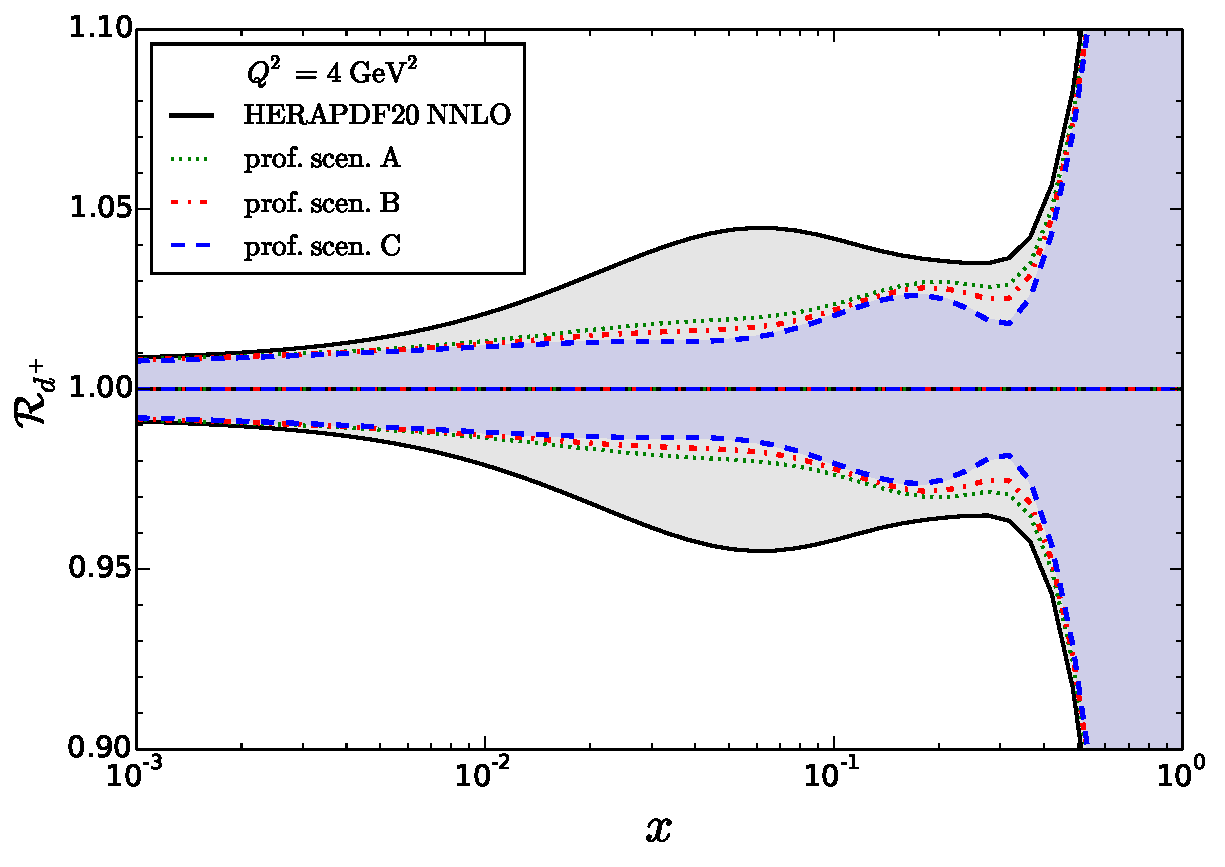
\includegraphics[width=0.45\textwidth]{plots/ratio_dPdbar_Q2.pdf}
\\
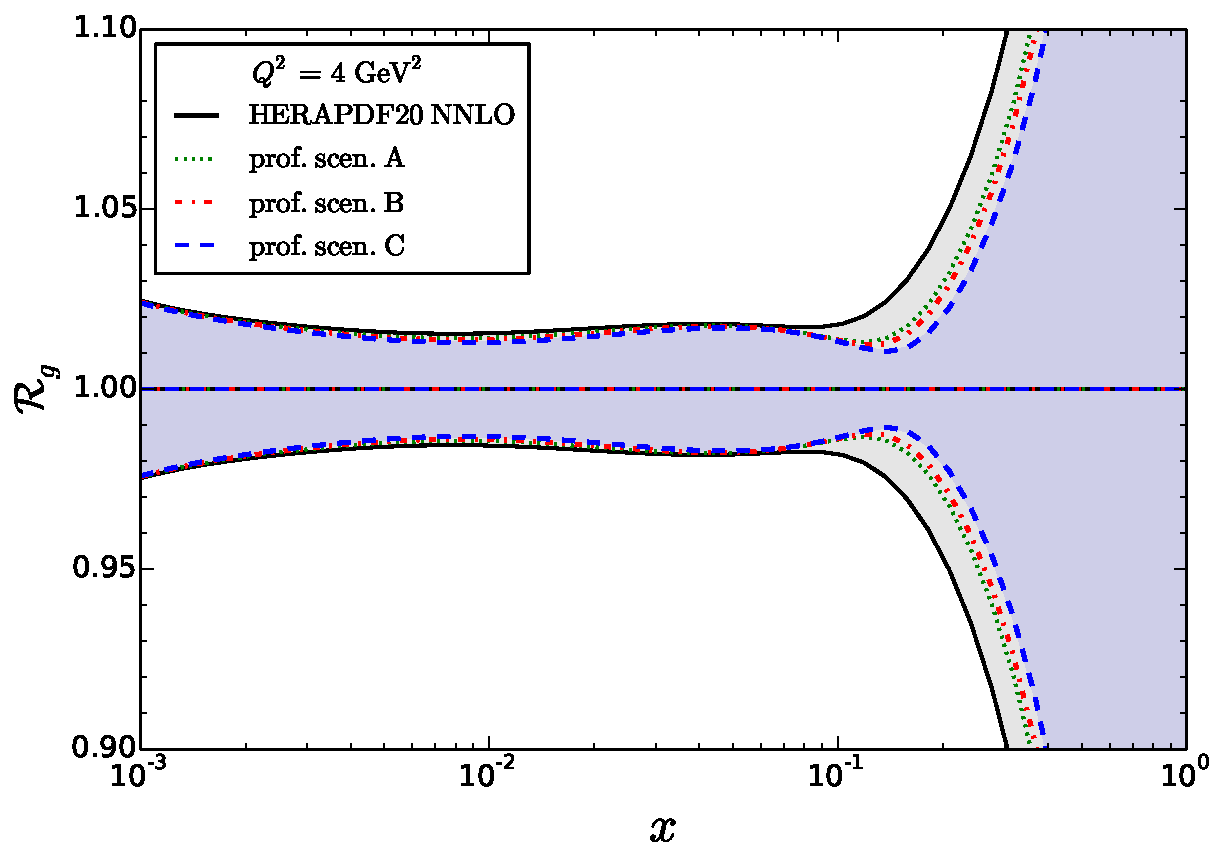
\includegraphics[width=0.45\textwidth]{plots/ratio_g_Q2.pdf}
%\\
%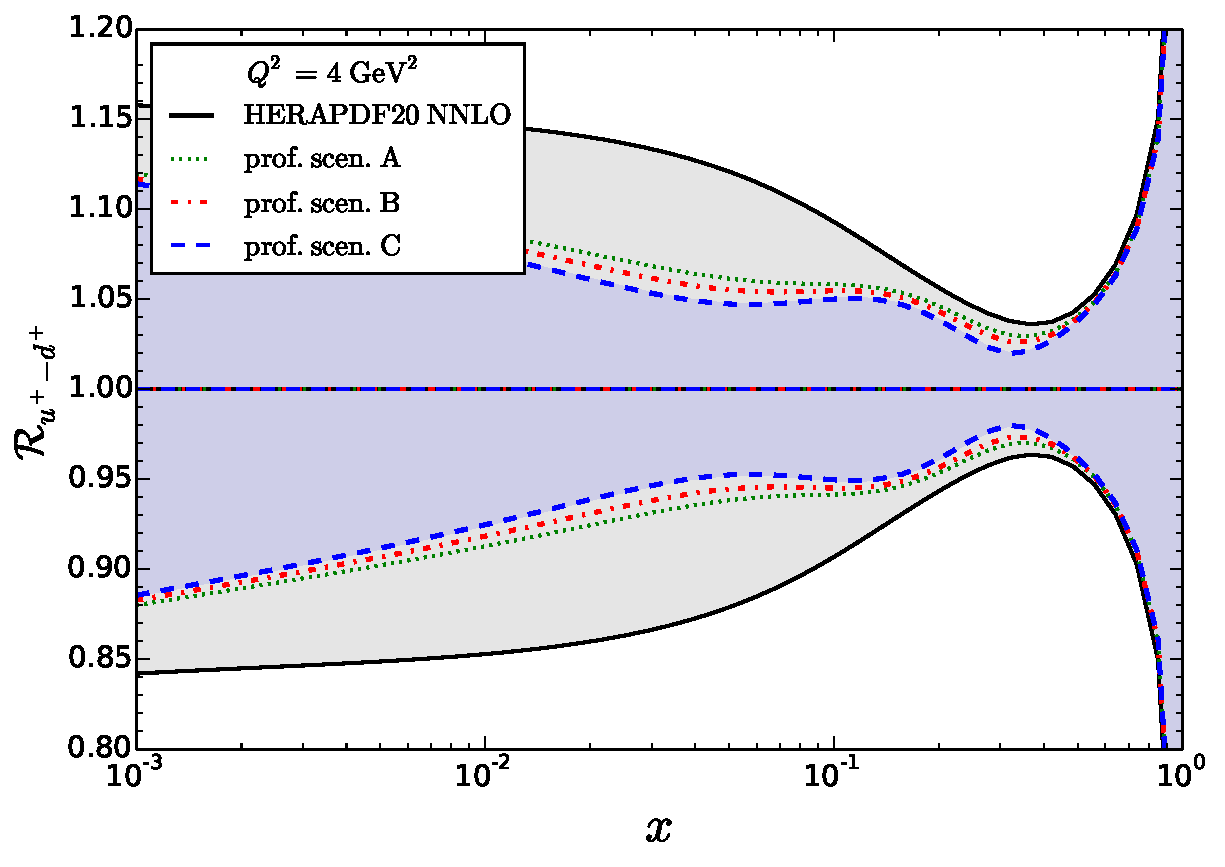
\includegraphics[width=0.3\textwidth]{plots/ratio_uPubarMdMdbar_Q2.pdf}
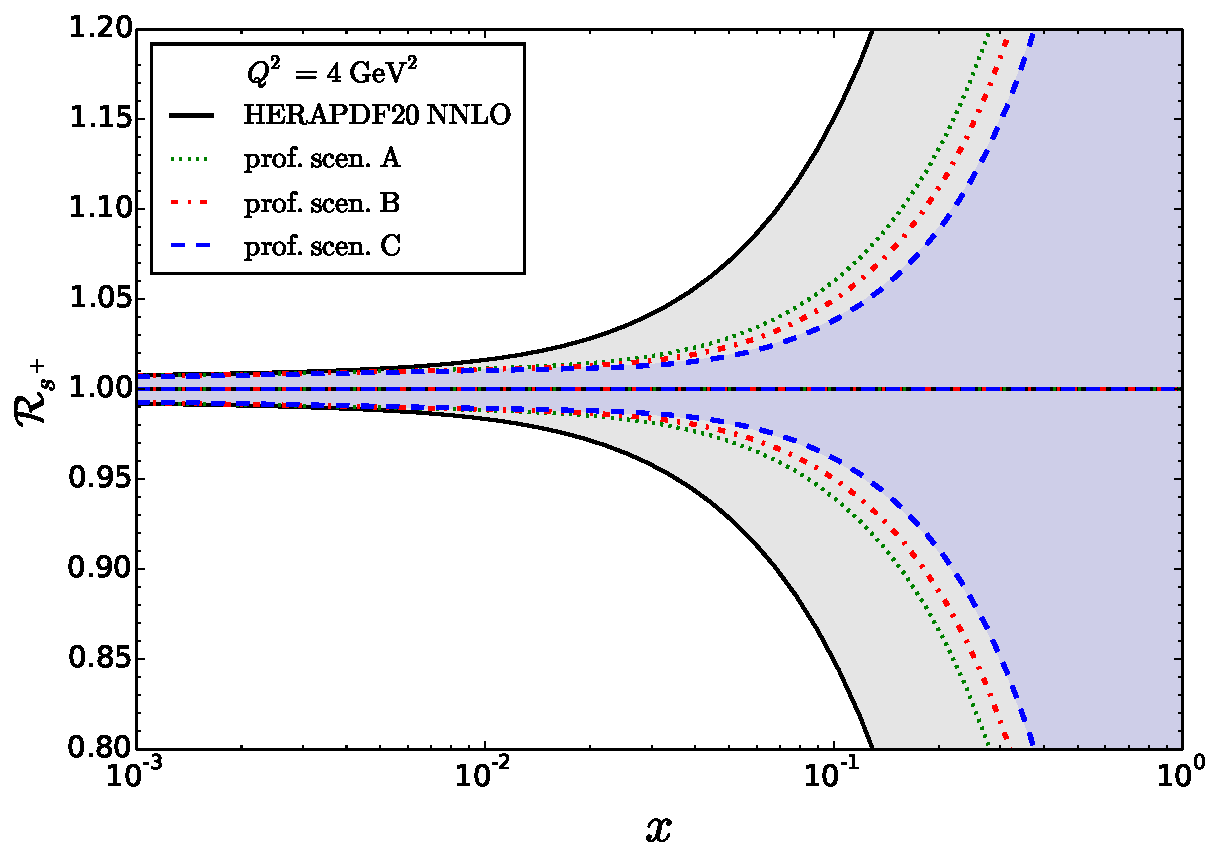
\includegraphics[width=0.45\textwidth]{plots/ratio_sPsbar_Q2.pdf}
\caption{\small Combinations of PDFs: $u^+$, $d^+$, $g$, $s^+$ at scale $Q^2=4$ GeV$^2$
for initial HERAPDF2.0 compared with the PDFs resulting from including Lattice moments
data in scenarios A, B and C.
%  \\
% \Red{NOTE: this is  an alternate figure. 
% I've dropped the $u^+-d^+$ so we can enlarge the figs and match the previous plot. 
% We need to pick ONE of the TWO figs. }
}
\label{fig:pdfsProf}
\end{figure}
%%%%%%%%%%%%%%%%%%%%%%%%%%%%%%%%%%%%%%%%%%%%%%%%%%%%%%%%


% 
% THIS IS THE OLD FIGURE WITH THE 5TH PLOT
% FRED' SUGGESTS JUST KEEPING 4 PLOTS
%
%   %%%%%%%%%%%%%%%%%%%%%%%%%%%%%%%%%%%%%%%%%%%%%%%%%%%%%%%%
%   %------------------------------------------------------
%   \begin{figure}[!t]
%   \centering
%   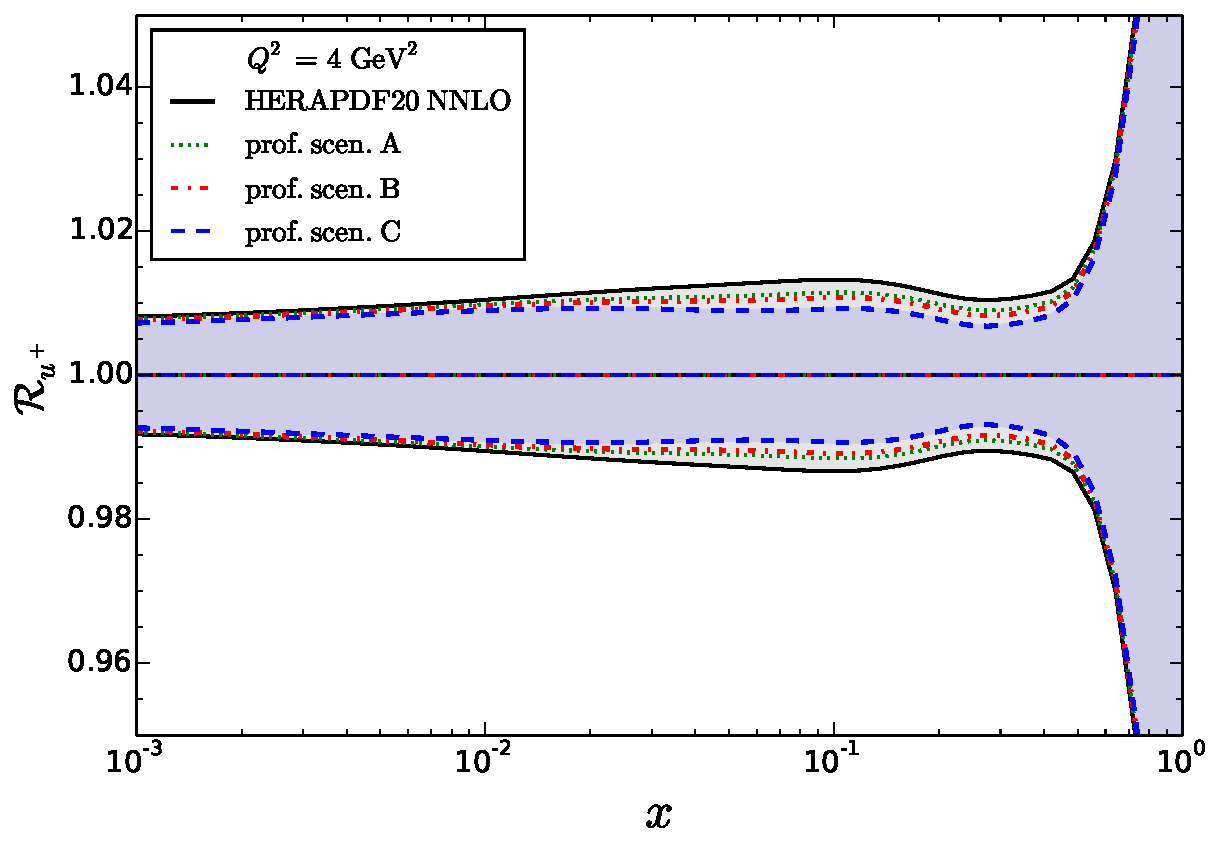
\includegraphics[width=0.3\textwidth]{plots/ratio_uPubar_Q2.pdf}
%   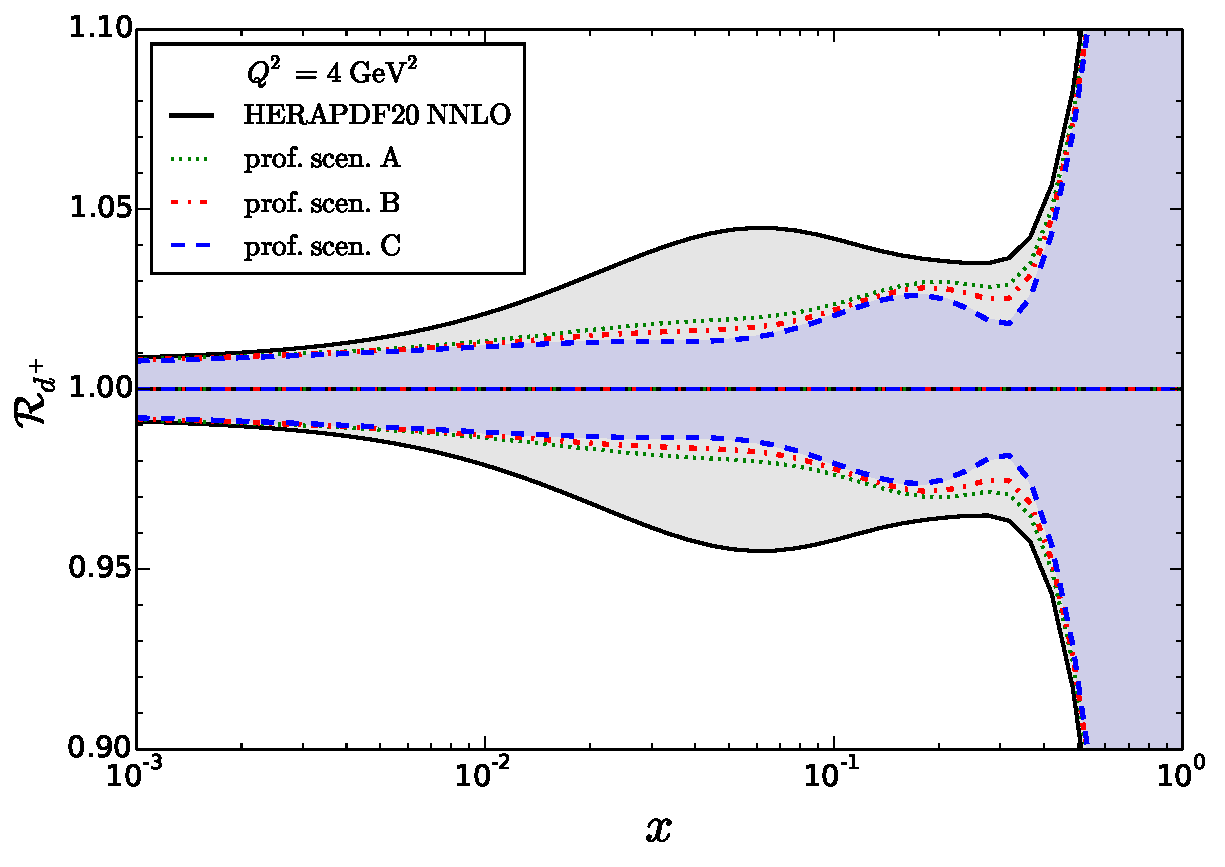
\includegraphics[width=0.3\textwidth]{plots/ratio_dPdbar_Q2.pdf}
%   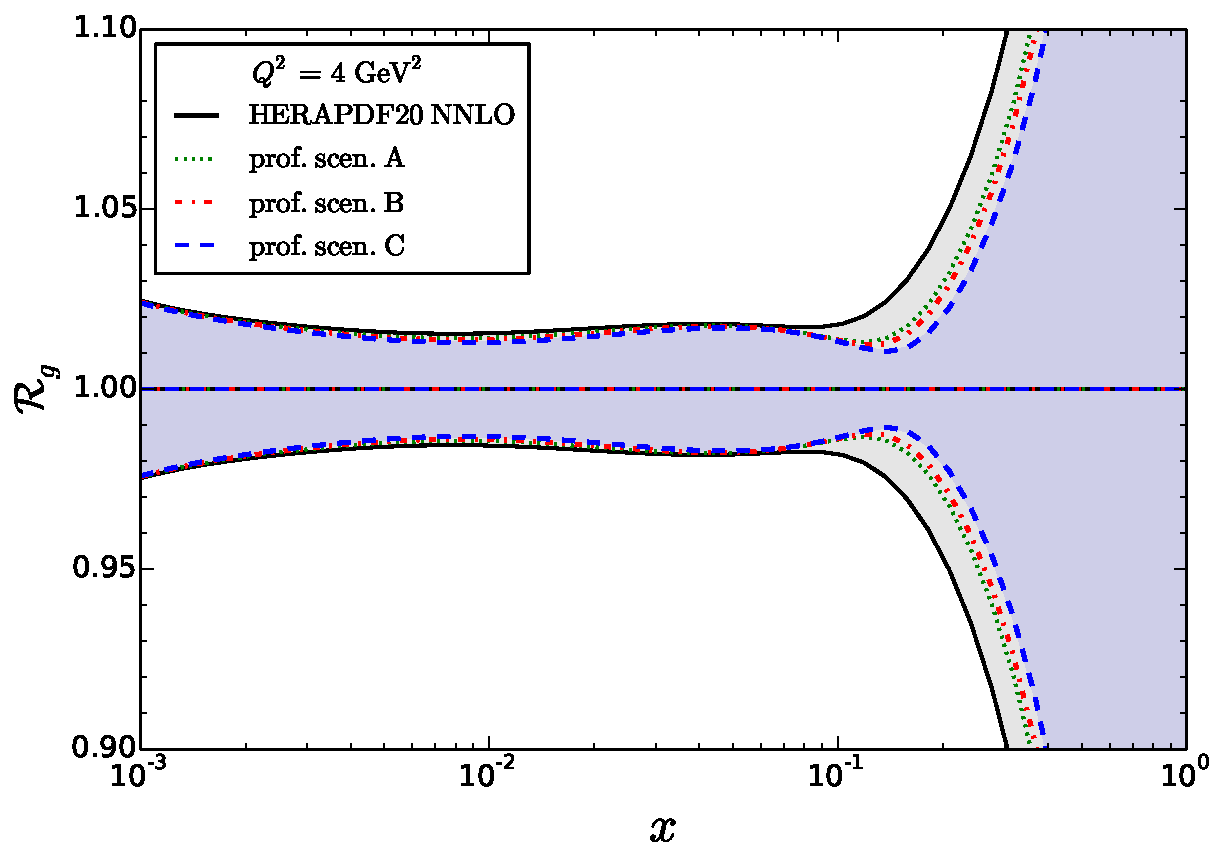
\includegraphics[width=0.3\textwidth]{plots/ratio_g_Q2.pdf}
%   \\
%   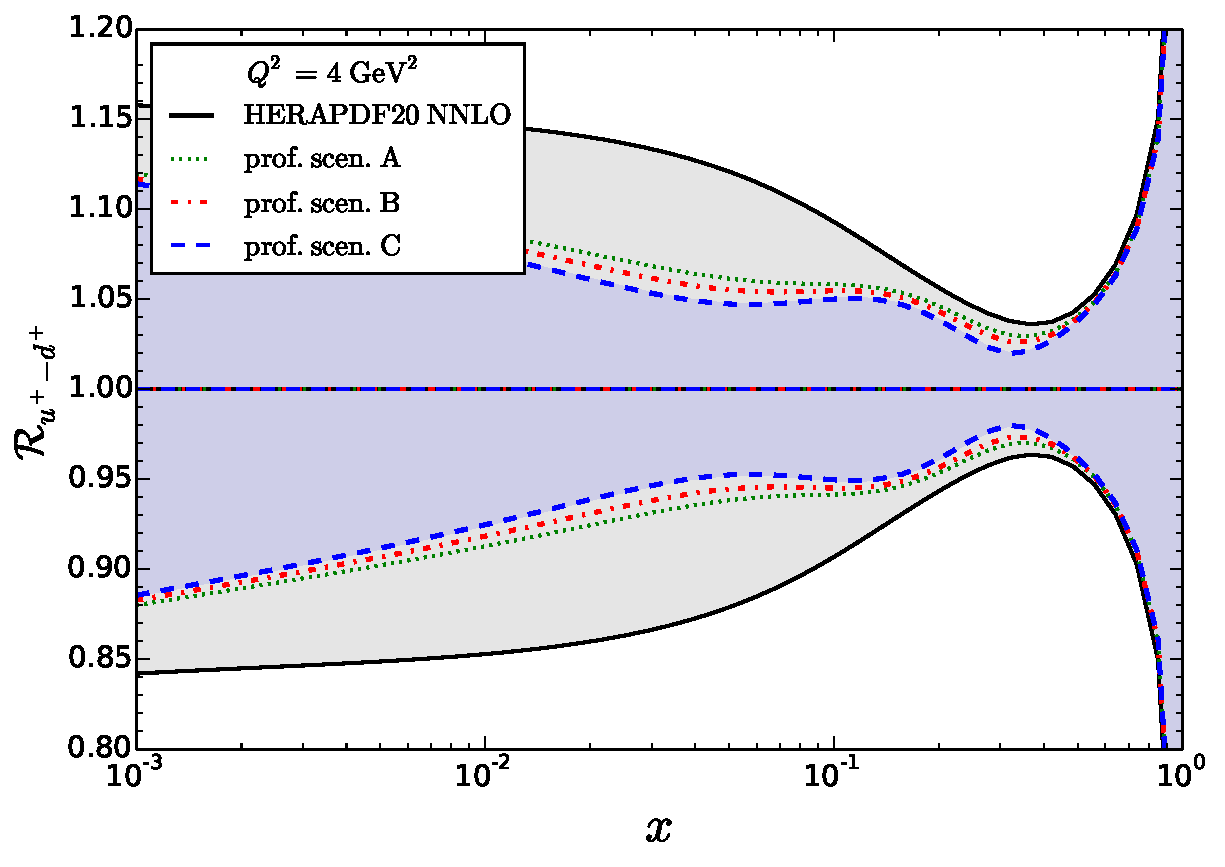
\includegraphics[width=0.3\textwidth]{plots/ratio_uPubarMdMdbar_Q2.pdf}
%   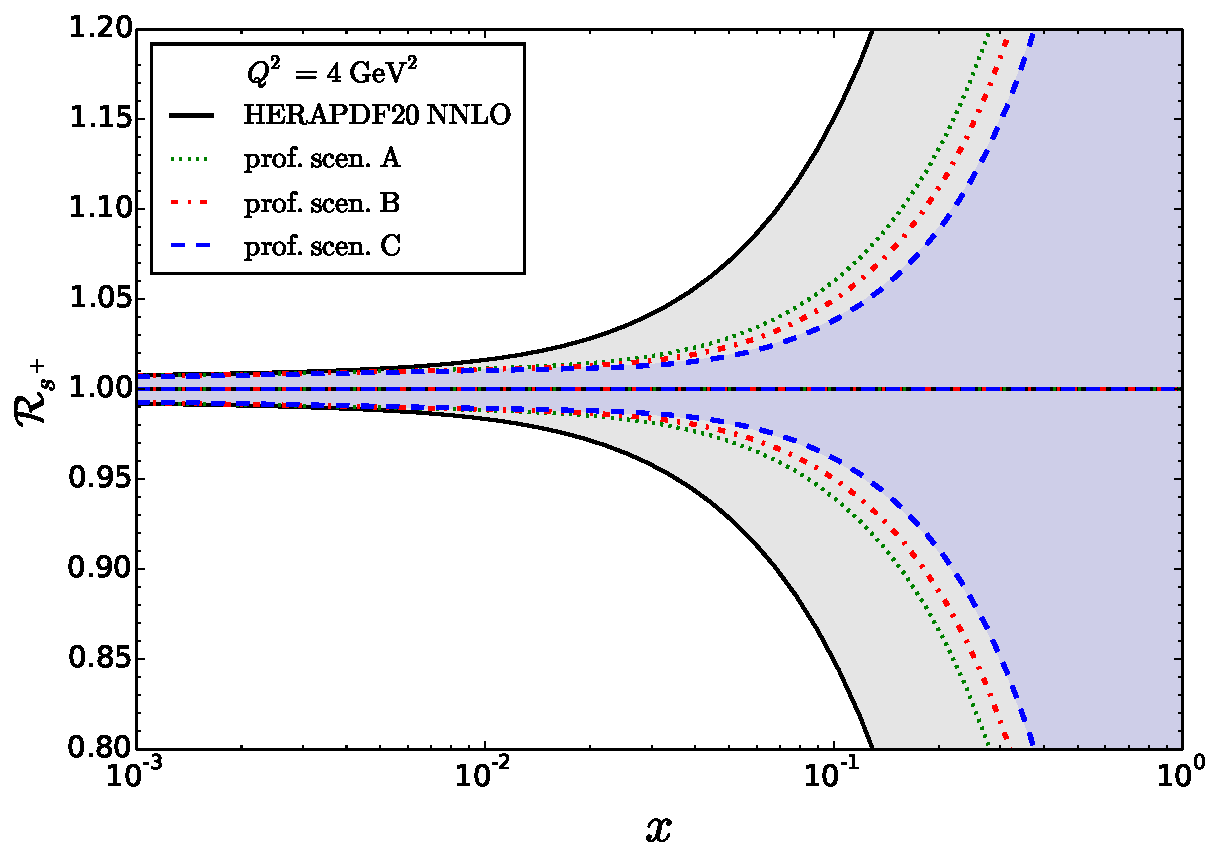
\includegraphics[width=0.3\textwidth]{plots/ratio_sPsbar_Q2.pdf}
%   \caption{\small Combinations of PDFs: $u^+$, $d^+$, $g$, $u^+-d^+$, $s^+$ at scale $Q^2=4$ GeV$^2$
%   for initial HERAPDF2.0 compared with the PDFs resulting from including Lattice moments
%   data in scenarios A, B and C.
%   }
%   \label{fig:pdfsProfOLD}
%   \end{figure}
%   %----------------------------------------------------------
%   %%%%%%%%%%%%%%%%%%%%%%%%%%%%%%%%%%%%%%%%%%%%%%%%%%%%%%%%





% x-space analysis using reweighting
\subsection{Impact of lattice calculations of  $x$-space PDFs}
\label{sec:projectionsxspace}

In the previous section, we studied the impact of
lattice-QCD calculations of PDF moments. 
%
We now perform an exploration of the
potential constraints that future lattice QCD calculations
of $x$-space PDFs can provide on global analyses.
%
We focus on the isotriplet
combination $x u-x d$ (and $x\Delta u - x\Delta d$
in the polarized case), the quark combination 
on which initial studies have been focused, as
it is the simplest to calculate, owing to the lack of disconnected
diagrams and the absence of mixing with other quark flavors or with gluons.


Following the same Bayesian reweighting procedure employed for PDF moments
in Sect.~\ref{sec:projections:rw},
we have generated pseudo-data for the isotriplet
combinations
\be
\label{eq:isotriplet_unpol}
u(x_i,Q^2)-d(x_i,Q^2) \, \quad{\rm and} \, \quad
\bar{u}(x_i,Q^2)-\bar{d}(x_i,Q^2) \, , \quad i=1,\ldots,N_x \, ,
\ee
for the unpolarized case, and for
\be
\label{eq:isotriplet_pol}
\Delta u(x_i,Q^2)-\Delta d(x_i,Q^2) \, \quad{\rm and} \, \quad
\Delta\bar{u}(x_i,Q^2)-\Delta\bar{d}(x_i,Q^2) \, , \quad i=1,\ldots,N_x \, ,
\ee
for the polarized case, with $N_x$ being the number of points
in $x$-space that are being sampled.
%
We take $Q^2=4$ GeV$^2$, consistent with our choices for the exercise 
performed in Sects.~\ref{sec:projections:rw}-\ref{sec:hessianprofiling}.

We consider three scenarios, denoted by scenario D, E, and F,
for the total uncertainty $\delta_L^{(i)}$
that will be assigned to
the lattice-QCD calculations of the specific quark
combinations listed in Eqs.~(\ref{eq:isotriplet_unpol})
and~(\ref{eq:isotriplet_pol}).
%
Lattice-QCD computations are expected to have the smallest systematic 
uncertainties at large $x$, so we choose the $N_x=5$ points to be
\be
x_i = 0.70\, ,0.75,\, 0.80,\, 0.85, \, 0.90 \, .
\ee
%
For each scenario, we assume the same relative error for each value of 
$\{x_i\}$, and we neglect possible correlations between 
neighbouring $x$-points.
%
We assume uncertainties of $\delta_{L}^{(i)}=12\%, 6\%$ and 3\% for scenarios
D, E, and F, respectively.
%
Note that we assume the same values of $\delta_{L}^{(i)}$ for the polarized
and unpolarized cases, as well as for both the quark
and the antiquark isotriplet combinations Eqs.~(\ref{eq:isotriplet_unpol})
and~(\ref{eq:isotriplet_pol}).

We summarize the results of this exercise in Fig.~\ref{fig:impactxspace}, 
where we plot the ratio of the PDF uncertainties in each scenario A, B and C 
(D, E and F) to the uncertainty of the original
NNPDF3.1 (NNPDFpol1.1) set.
%
We show the impact on the PDF uncertainties
in $\bar{u}$ and $\bar{d}$ at large-$x$ in the upper
plots, with the corresponding comparison for $\Delta\bar{u}$
and $\Delta\bar{d}$ in the lower plots.
%
We concentrate on the results for the individual quark flavors, even though 
the constraints are imposed on differences between flavors, as the former are 
of the more direct interest for phenomenology. 
%
From this comparison, we find that lattice-QCD calculations of the 
$x$-dependence of PDFs can significantly reduce the uncertainties for both 
unpolarized and polarized antiquarks in the large-$x$ region.
%
Taking into account that the PDF uncertainties on the large-$x$
antiquarks are rather large, and that they
enter a number of important Beyond Standard Model (BSM) search channels
(such as for instance for production of new heavy gauge bosons $W'$ and $Z'$),
our analysis demonstrates that such calculations would have direct
phenomenological implications.
%
In a Monte Carlo approach such as NNPDF, the
PDF uncertainties themselves fluctuate, particularly at low-scales,
explaining the wiggles in these plots.

%-------------------------------------------------------------------
\begin{figure}[!t]
\centering
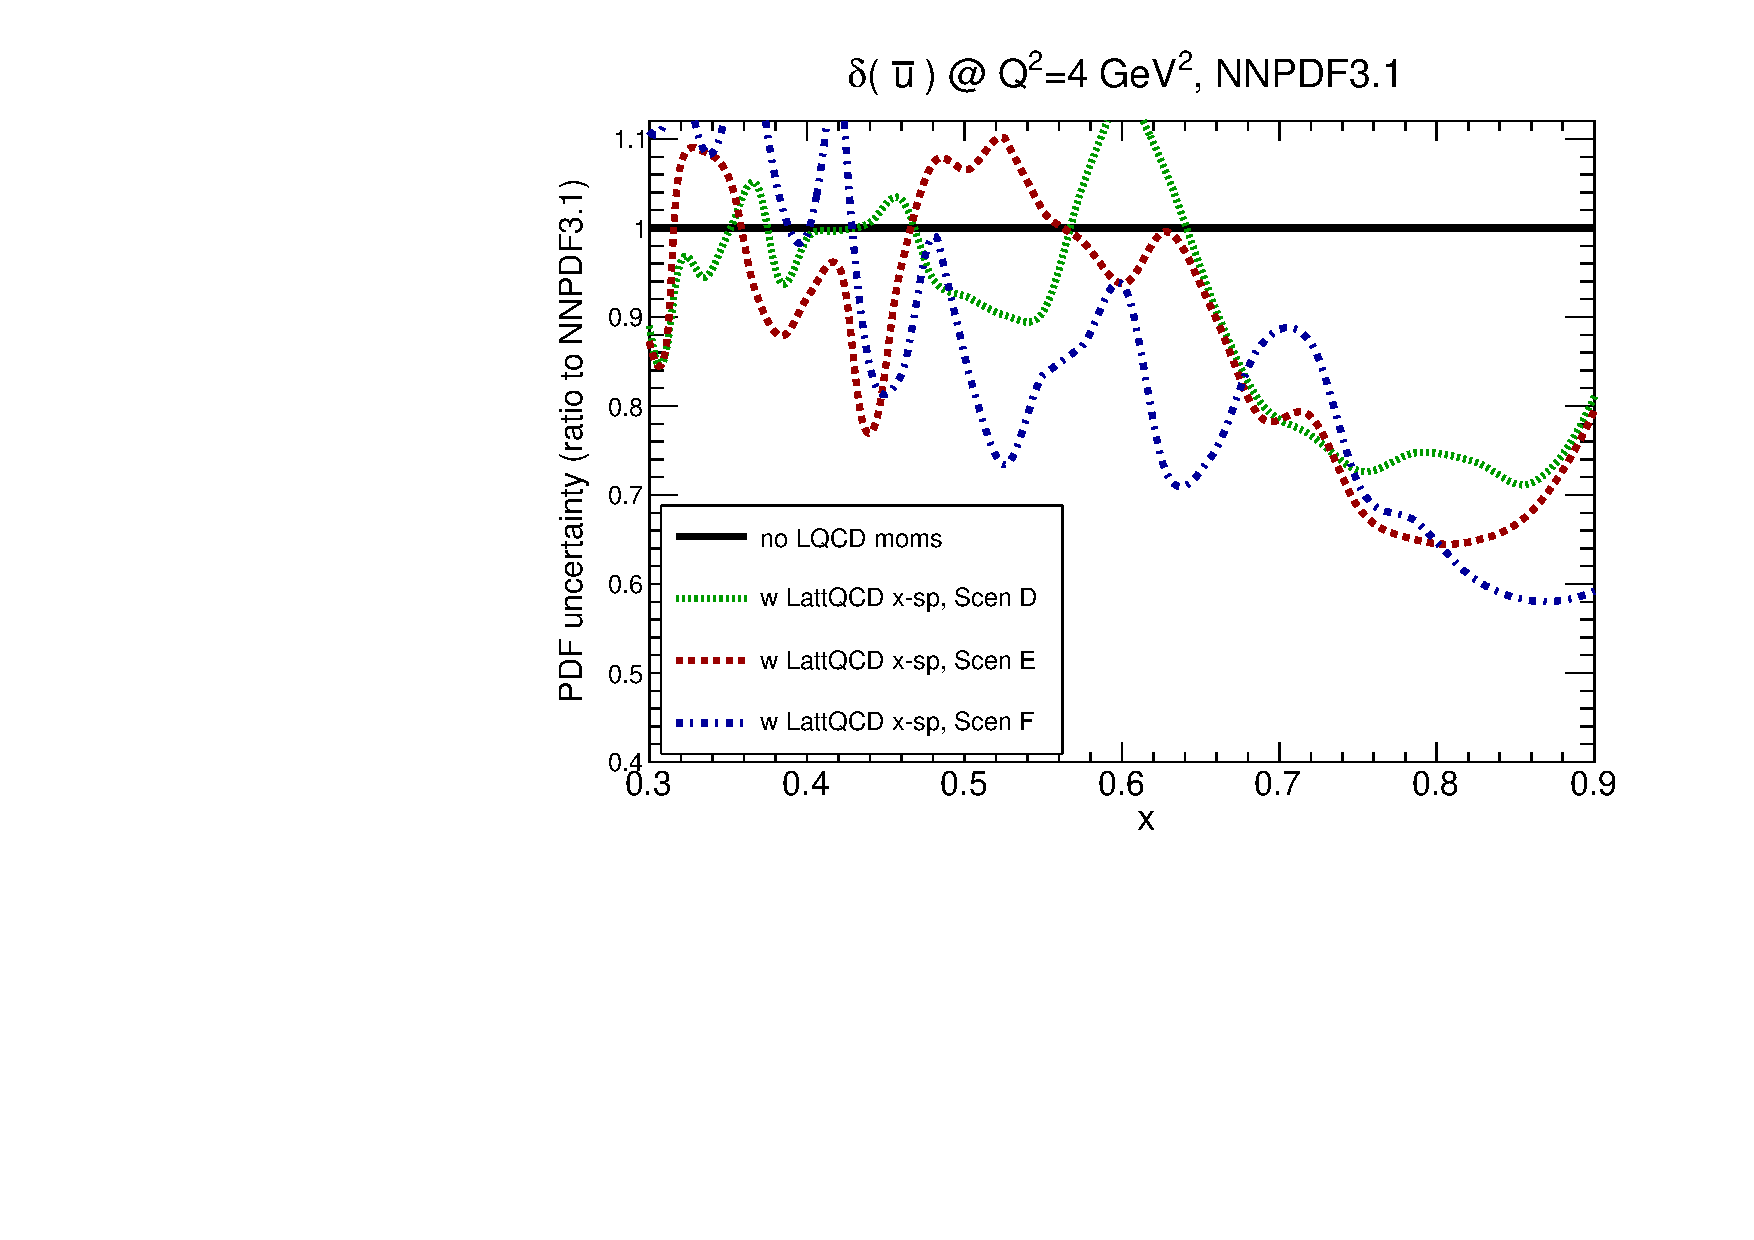
\includegraphics[scale=0.45]{plots/xubar-unpol-lattice-relerr-xdata-xspace.pdf}
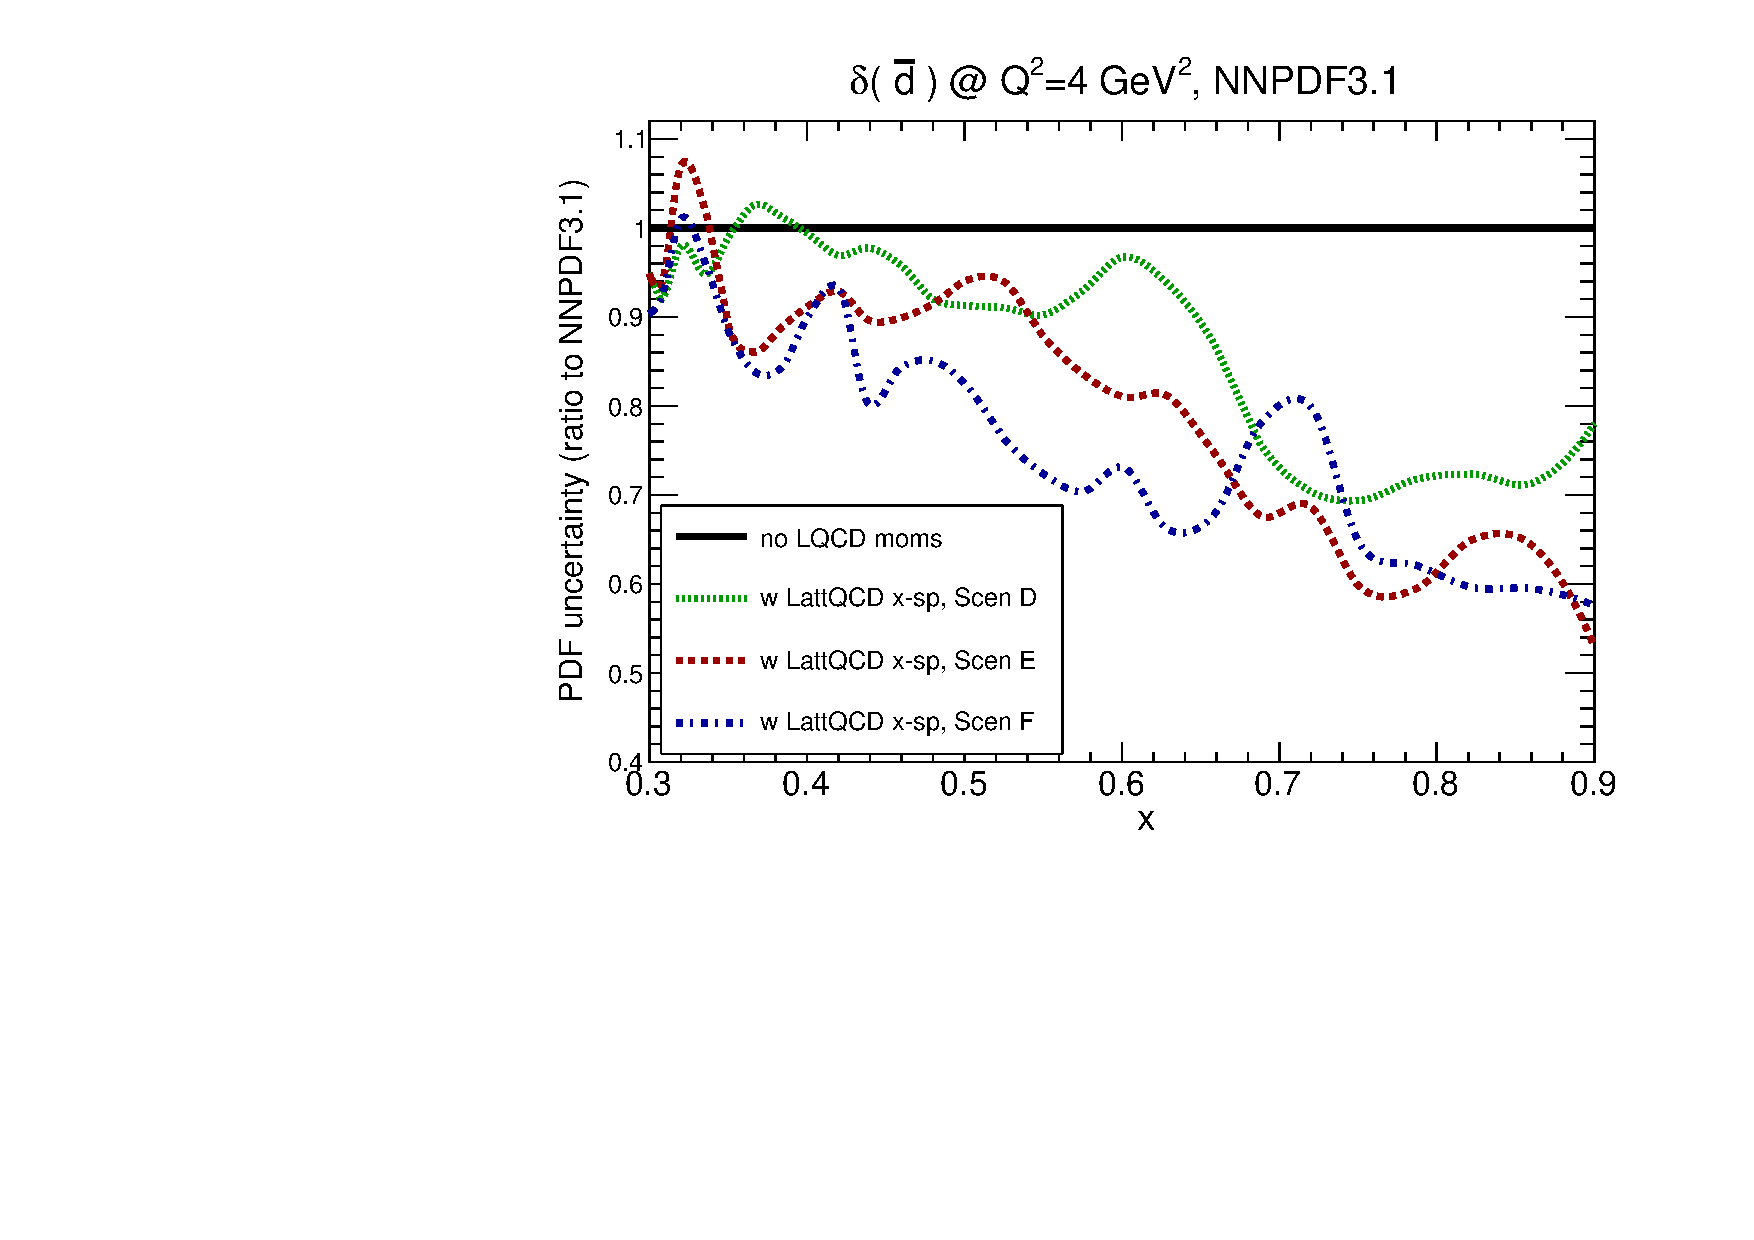
\includegraphics[scale=0.45]{plots/xdbar-unpol-lattice-relerr-xdata-xspace.pdf}
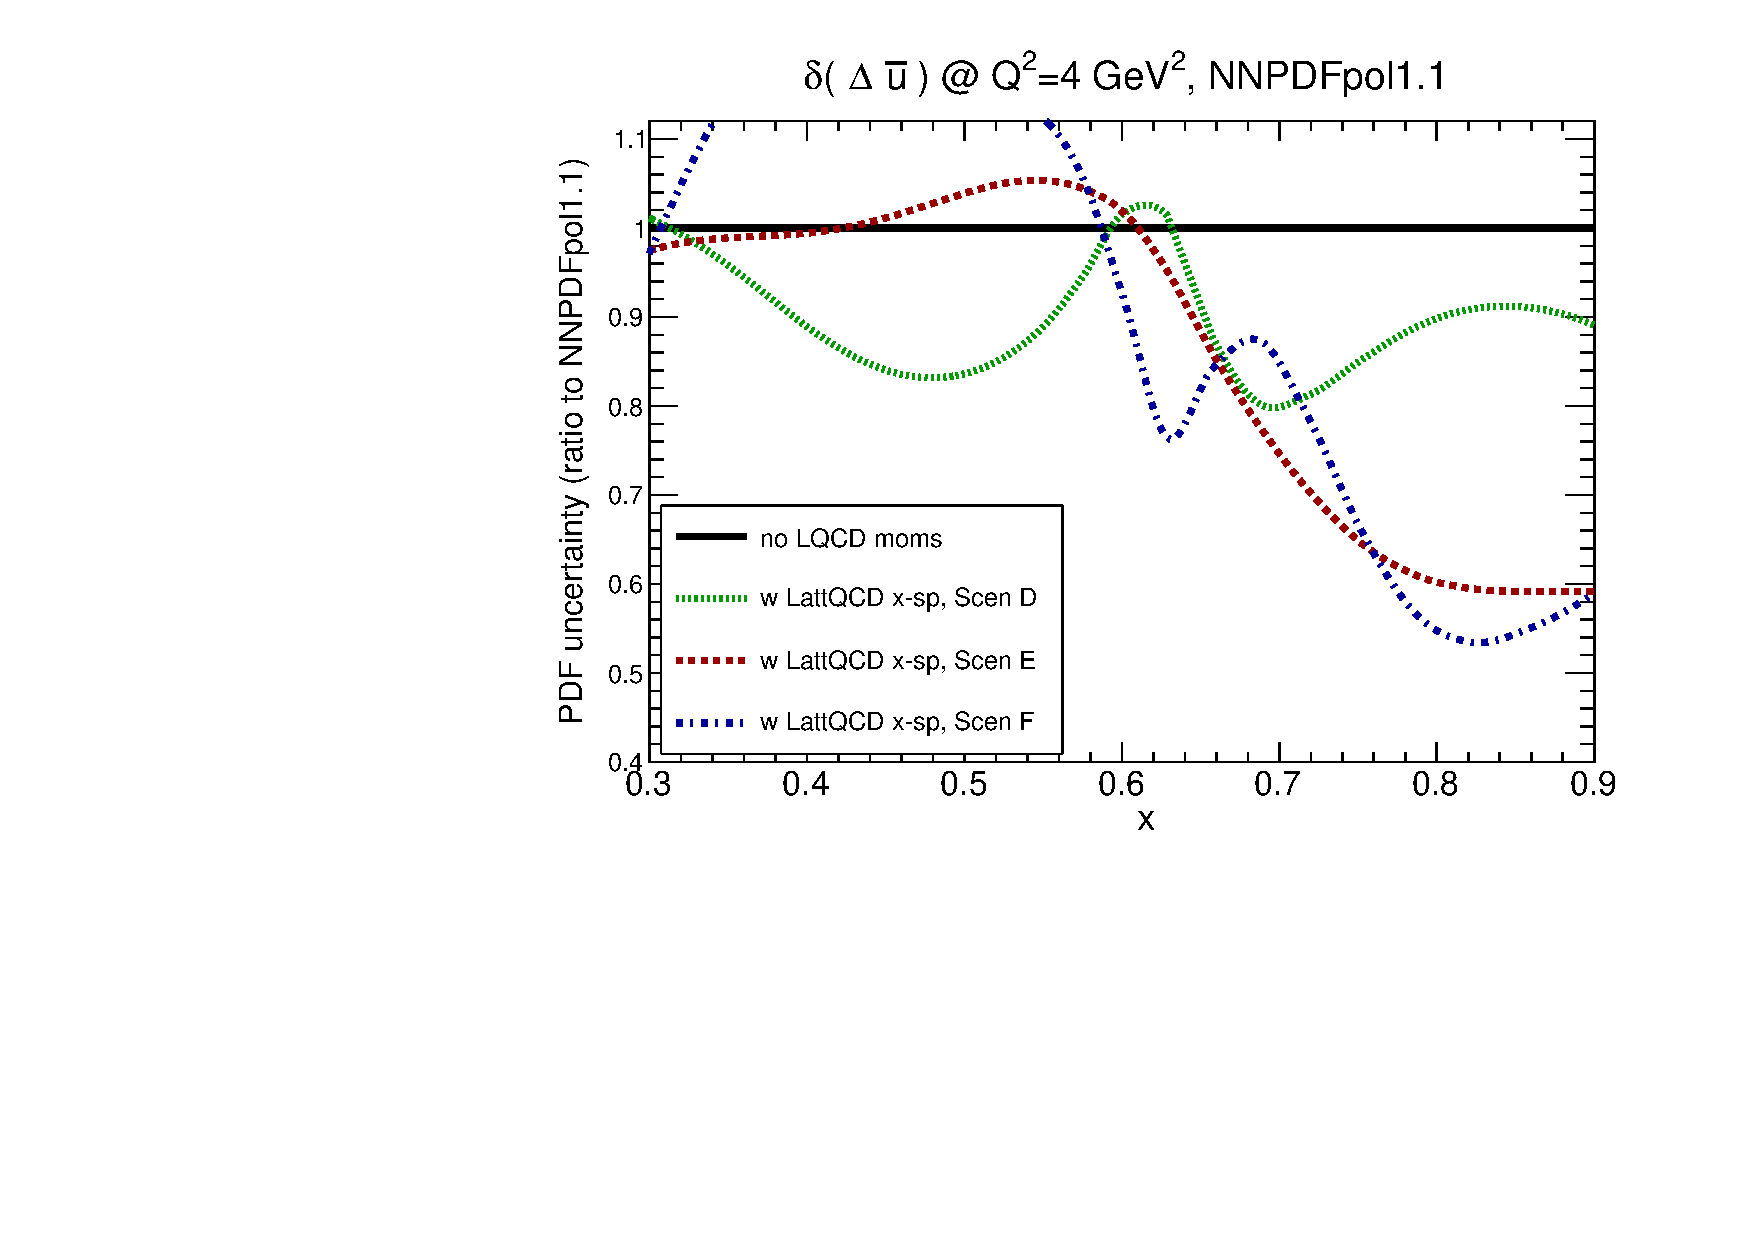
\includegraphics[scale=0.45]{plots/xubar-pol-lattice-relerr-xdata-xspace.pdf}
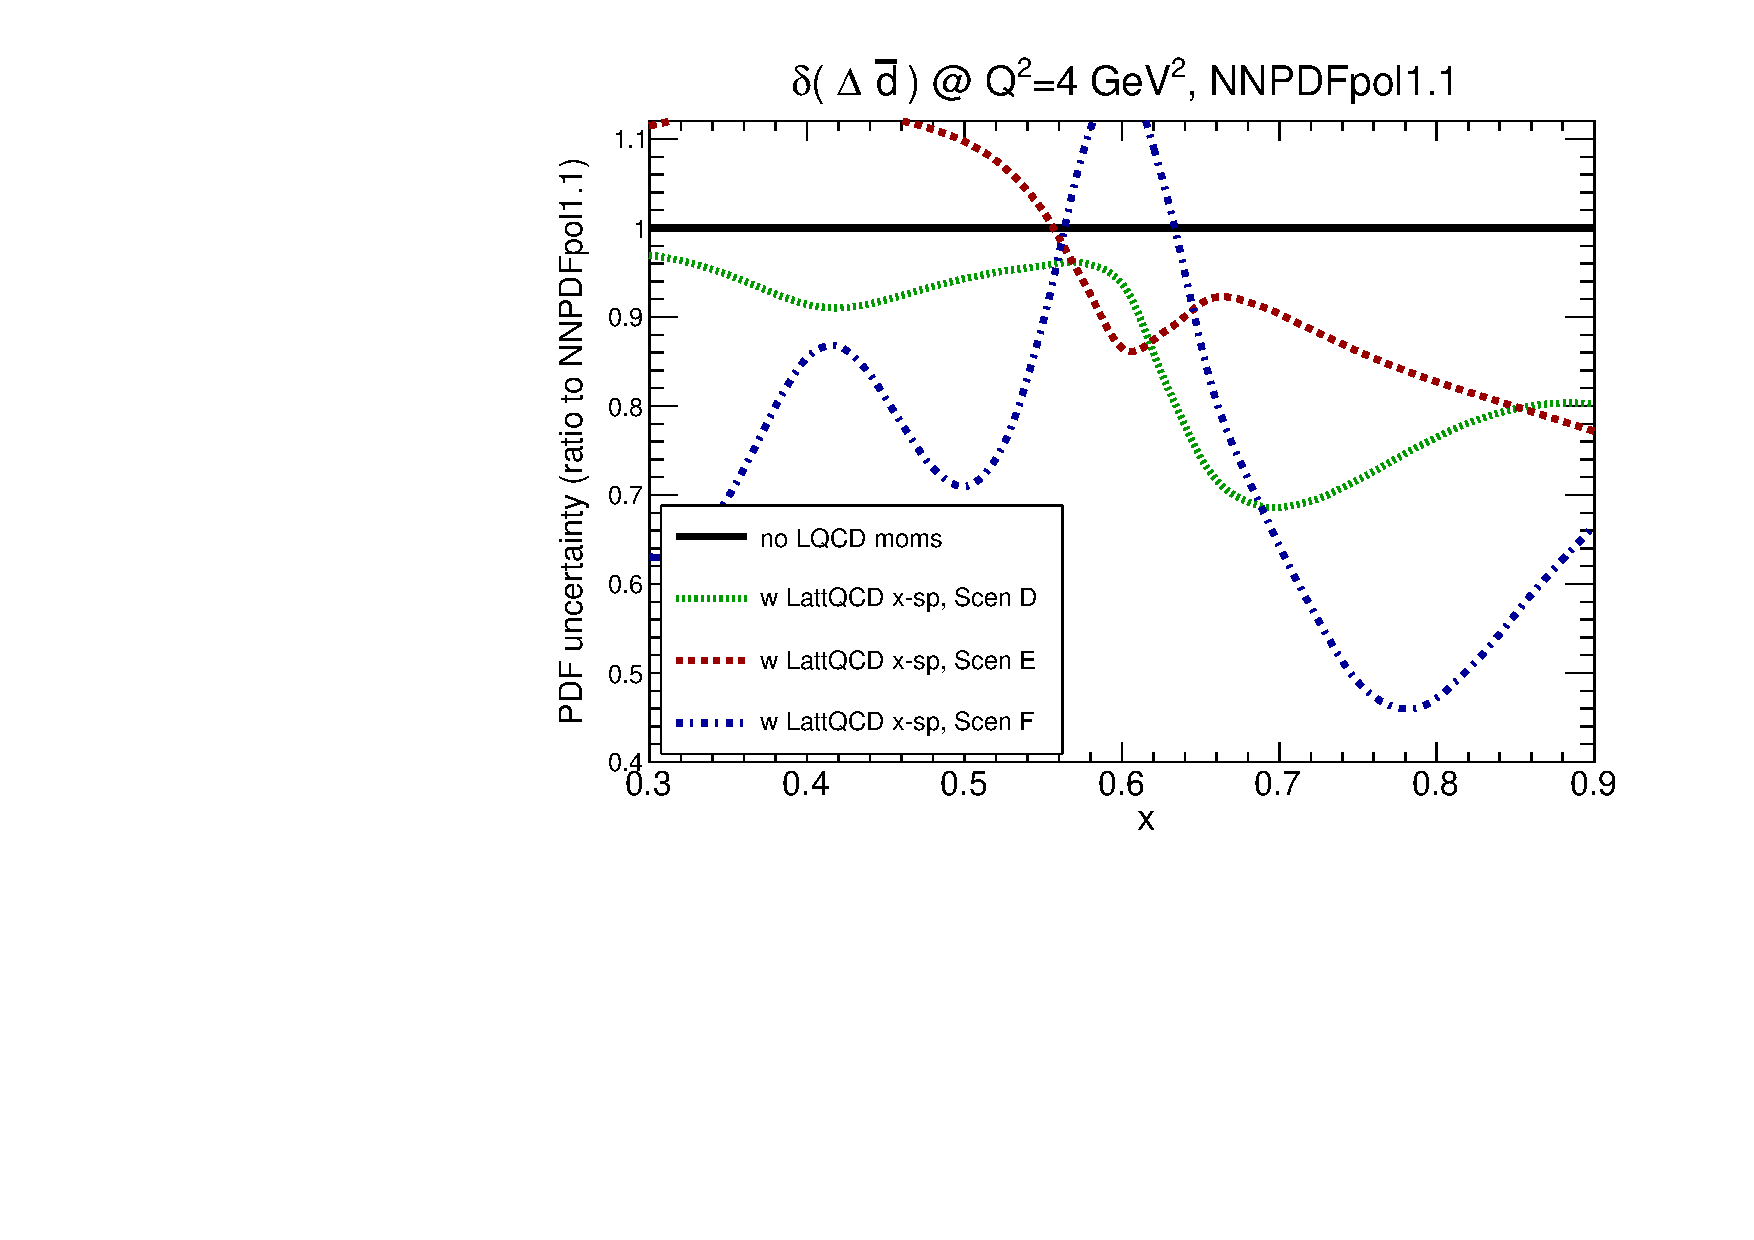
\includegraphics[scale=0.45]{plots/xdbar-pol-lattice-relerr-xdata-xspace.pdf}
\caption{\small The ratio of PDF uncertainties to the original
  NNPDF3.1 (NNPDFpol1.1) in the fits where lattice-QCD pseudo-data
  on $x$-space PDFs have been added to the global unpolarized
  (polarized) analysis.
  %
  Specifically, we show the impact on the PDF uncertainties
  in $\bar{u}$ and $\bar{d}$ at large-$x$ in the upper
  plots, with the corresponding comparison for $\Delta\bar{u}$
  and $\Delta\bar{d}$ in the lower plots.
}    
\label{fig:impactxspace}
\end{figure}
%---------------------------------------------------------------------

Fig.~\ref{fig:impactxspace} shows that
in the unpolarized case the large-$x$ PDF uncertainties could be reduced
to $60\%$ of their original value.
%
We also find that there are no large
differences between the three
scenarios,
probably because the constraint is on quark differences not on individula 
flavors, so there is freedom for $\bar u$ and $\bar d$ to vary in a correlated 
fashion while still satisfying the constraint. 
%
However, it does suggest 
that a direct lattice-QCD calculation
of $x \bar{u}-x \bar{d}$ does not need to reach uncertainties
at the few-percent level to influence global fits.
%
For the polarized PDFs, Fig.~\ref{fig:impactxspace} demonstrates that the
reduction in PDF uncertainties could be significantly more marked.
%
For instance, in the case of $\Delta \bar{d}$, at $x\simeq 0.8$
the resulting PDF uncertainty from scenario F is less than 50\%
of the original uncertainty.

In Tab.~\ref{tab:neffxspace} we indicate the effective number of replicas
$N_{\rm eff}$, Eq.~(\ref{eq:effnrep}), remaining when
the lattice-QCD pseudo-data for Eqns.~(\ref{eq:isotriplet_unpol})
and~(\ref{eq:isotriplet_pol}) are included in the global
unpolarized and polarized fits.
%
Here we find a marked decrease in $N_{\rm rep}$
for the three scenarios,
in particular for the unpolarized case.
%
For example, in the most optimistic scenario F, only
64 effective replicas remain out of the
original sample of $N_{\rm rep}=1000$ replicas.
%
See Tab.~\ref{tab:neff} for the corresponding
information at the level of PDF moments.
   
%------------------------------------------------------------------------------
\begin{table}[!t]
\centering
\footnotesize
\renewcommand{\arraystretch}{1.3} 
\begin{tabular}{lcc}
\toprule
&  NNPDF3.1  &  NNPDFpol1.1 \\
\midrule
$N_{\rm rep}$ original   & 1000 & 100 \\
$N_{\rm eff}$ Scenario D &  376 &  41 \\
$N_{\rm eff}$ Scenario E &  173 &  35 \\
$N_{\rm eff}$ Scenario F &  64  &  22 \\
\bottomrule
\end{tabular}
\caption{\small The effective number of replicas
  $N_{\rm eff}$, Eq.~(\ref{eq:effnrep}), remaining when the pseudo-data
  on the lattice-QCD calculations
  of Eqns.~(\ref{eq:isotriplet_unpol})
  and~(\ref{eq:isotriplet_pol}) 
  are included in the global
  unpolarized and polarized fits. 
  \label{tab:neffxspace}
  }
\end{table}
%-------------------------------------------------------------------------------

We emphasize that the results of this exercise must be interpreted
with some care.
%
First of all, the results depend sensitively on the specific values of
$\left\{ x_i \right\}$
that we have assumed for the lattice-QCD calculation,
and on the values
of the associated uncertainties $\delta_L^{(i)}$.
%
The quantitative results depend on the choice of input PDF set and would 
vary if, for example, the input set were the HERAPDF2.0 set used for the 
Hessian profiling exercise of Sect.~\ref{sec:hessianprofiling}.
%
Even with these caveats, our analysis makes clear that a direct
computation of the isotriplet combination $x u-x d$ on the lattice
has the potential to constrain the large-$x$ PDFs in
a more significant way than corresponding PDF moment calculations,
particularly in the unpolarized case.
%
Given the importance of antiquark PDFs in the large-$x$ region for LHC 
phenomenology (especially for a high-luminosity run), 
pursuing these calculations should be high on the list
of priorities for the lattice-QCD community.




% General discussion
\subsection{Discussion}

We conclude this section with a brief discussion of the main lessons that
can be learned from this exercise, which provides the first quantitative 
estimate of the impact of present and future lattice-QCD calculations of PDF 
moments and $x$-space PDFs, for both polarized and unpolarized PDFs.

First, we have demonstrated that in the polarized case,
even with current uncertainties, lattice-QCD calculations of
selected PDF moments can impose sizable constraints on several
important polarized quark combinations.
%
This suggests that global polarized PDF analyses should consider
including existing lattice-QCD calculations in their fits to constrain some
of the least known quark combinations, such as the total strangeness.
%
The situation is rather different in the unpolarized case,
where a reduction of the current lattice-QCD uncertainties by a factor of 
between five and ten seems to be required to influence global fits.
%
This difference arises because unpolarized PDFs are known with much higher 
precision than polarized PDFs, thanks to the much wider amount of experimental 
data sensitive to unpolarized PDFs,
including the constraints from recent high-precision measurements at the LHC.
%
Thus, in addition to the differences highlighted  in Fig.~\ref{fig:Bmomsunp},
much more precise lattice-QCD calculations than in the polarized case 
need to be used to be competitive with current PDF fits.


Second, lattice-QCD calculations of the quark isotriplet combinations
$xu-xd$ and $x\bar{u}-x\bar{d}$ would be instrumental in constraining
quark PDFs at large $x$.
%
Even a calculation with $\delta_L\simeq 10\%$ uncertainties at large-$x$ would
start to provide useful constraints on global fits.
%
Moreover, we find that, in the unpolarized case, the information on the
PDFs that could be derived from a direct $x$-space calculation
from lattice-QCD is clearly superior to the information that can be obtained
from PDF moments alone, at least for the subset of PDFs and moments used in 
the present exercise.

The profiling studies presented in this section could be extended in
a number of directions.
%
In the polarized case, one could include the current lattice-QCD
values of the moments listed in Tab.~\ref{tab:BMpol} in global analyses: 
indeed, we have demonstrated that at the current level of uncertainties one 
expects to find some non-trivial constraints.
%
In this respect, a crucial topic to investigate is the compatibility 
(or lack thereof) of the existing lattice-QCD numbers compared to constraints 
from experimental data.
%
For both unpolarized and polarized PDFs, it would be interesting to include the 
effects of other moments and flavor combinations.
%
Higher moments, in particular, typically probe regions of higher $x$, compared
to lower moments, and in the large-$x$ regions uncertainties in the global-fit 
PDFs are more marked.
%
One could also consider the effects of the quark combinations for which 
$x$-space calculations might be available, for example those related to the 
proton strangeness.
%
Finally, a more refined analysis should include the theoretical correlations
expected in lattice-QCD calculations, for instance, in the case of $x$-space 
calculations, one expects neighboring points in $x$ to be highly correlated.



